\documentclass[12pt,twoside,openright]{extarticle}

\usepackage[T1]{fontenc}
\usepackage{polski}
\usepackage[utf8x]{inputenc}
\usepackage[polish]{babel}
\usepackage{url}
\usepackage{afterpage}

\usepackage[margin=1.3in]{geometry}
\usepackage{color}
\usepackage{graphicx}
\usepackage{float}
\usepackage{indentfirst}
\usepackage[nottoc,notlot,notlof]{tocbibind}
\usepackage{varwidth}
\setlength\parindent{1cm}
\raggedbottom

\usepackage{listings}
\renewcommand{\lstlistingname}{Kod}
\lstset{
	language=Java,
	basicstyle=\ttfamily,
	numbers=left,
 	numberstyle=\tiny,
	frame=tb,
	tabsize=4,
	columns=fixed,
	showstringspaces=false,
	showtabs=false,
	keepspaces,
	commentstyle=\color{red},
	keywordstyle=\color{blue}
}

\usepackage[hidelinks]{hyperref}
 
\newtheorem{theorem}{Problem}

\begin{document}
\begin{titlepage}
    \begin{center}
        
\includegraphics[width=4cm]{polsl.png}\\[1cm]
        \textsc{\LARGE{Politechnika Śląska}}\\[0.5cm]
        \textsc{\LARGE{Wydział Automatyki, Elektroniki i~Informatyki}}\\[0.5cm]
        \textsc{\LARGE{Kierunek Informatyka}}\\[2.5cm]
        \LARGE{Praca magisterska}\\[1cm]
        \begingroup
            \fontsize{14pt}{17pt}\selectfont
            Analiza porównawcza przetwarzania strumieniowego w Java 8 \\ i realizacji zapytań SQL w pamięci
        \endgroup
    \end{center}
    \vspace{2cm}
    \begingroup
        \fontsize{14pt}{17pt}\selectfont
        \textbf{Autor:} Aleksander Grzybowski\\
        \textbf{Kierujący pracą:} dr inż. Ewa Płuciennik\\
    \endgroup

    \vspace{2.0cm}
    \begingroup
        \fontsize{12pt}{14pt}\selectfont
        \begin{center}
        Gliwice, czerwiec 2017
        \end{center}
    \endgroup
\end{titlepage}

\clearpage\mbox{}\clearpage

\tableofcontents

\newpage

\section{Wstęp}

    Dział informatyki zajmujący się przetwarzaniem danych zajmuje ważne miejsce w obszarze nauk informatycznych. W każdym programie obliczeniowym dobór odpowiednich mechanizmów gromadzenia i przetwarzania informacji znacząco wpływa na jego wydajność. Dotyczy to zwłaszcza systemów gromadzenia danych wielkiej skali (tzw. \textit{Big Data}), które bardzo często wymagają przetwarzania w czasie zbliżonym do rzeczywistego.

    Najpopularniejszym sposobem na gromadzenie danych są sprawdzone bazy relacyjne, wykorzystujące język SQL. Od wielu lat rozwiązania relacyjne wykorzystywane są we wdrożeniach różnorakiej skali, od małych aplikacji osobistych po klastry obliczeniowe. Niestety, korzystanie z baz relacyjnych w aplikacjach opartych o języki obiektowe jest zwykle problematyczne i wymaga wykorzystywania dodatkowych warstw pośrednich, np. metod mapowania obiektowo-relacyjnego. Pojawienie się wśród dostępnych rozwiązań języka Java w wersji 8 oraz nowo wprowadzonego Stream API, pozwalającego na wydajne i łatwe przetwarzanie danych z wykorzystaniem mechanizmów równoległych, zwiększyło liczbę możliwych metod, które można rozważyć przy wyborze technologii. Pojawia się pytanie, czy jest możliwe wykorzystanie strumieni do przetwarzania danych w sposób natywny dla języka w podobny sposób.

	Celem niniejszej pracy magisterskiej jest porównanie możliwości przetwarzania danych w bazach wykorzystujących język SQL z metodami dostarczanymi przez Stream API. Badania obejmują eksperymenty wydajnościowe, przeprowadzone w zakresie metod przechowywania danych w pamięci RAM, jak i obserwacje sposobów formułowania kodu i możliwości języka zapytań. W ramach pracy stworzone zostało środowisko badawcze, zaimplementowane w języku Java, oraz zaproponowano i wykonano zbiór testów wydajnościowych.

    Niniejsza praca składa się z 6 rozdziałów. Rozdział 2 zawiera szczegółową charakterystykę Stream API, przykłady użycia oraz szczegóły implementacyjne w kontekście przetwarzania równoległego. Rozdział 3 opisuje różnice pomiędzy metodami, odpowiedniki operacji w obu metodach, wewnętrzną reprezentację pamięciową danych oraz format wynikowy zapytania. Rozdział 4 zawiera wyniki oraz wnioski z badań wydajnościowych wykonanych przy użyciu danych syntetycznych, przeprowadzonych na obu rozwiązaniach bazodanowych. Rozdział 5 zawiera szczegóły testu referencyjnego TPC-H oraz opis sposobu jego implementacji i uruchomienia. Rozdział 6 zawiera podsumowanie prac, całościowe wnioski oraz propozycje przyszłych badań. Dokumentacja środowiska badawczego oraz wymagania sprzętowo-programowe zawarte są w dodatku A.

\cleardoublepage
\section{Analiza dziedziny}
    Niniejszy rozdział opisuje cechy i zastosowania pamięciowych baz SQL oraz podstawowe cechy Stream API, wraz z przykładami jego wykorzystania przy uwzględnieniu przetwarzania równoległego.

    Bazy danych SQL są powszechnie stosowanymi rozwiązaniami do gromadzenia i odczytu danych. Struktura danych ściśle określona przez definicje tabel, ochrona integralności poprzez ograniczenia i więzy referencyjne oraz wygodny język SQL zachęcają do ich stosowania zarówno dla małych, jak i dużych zbiorów danych. Mimo pojawienia się nowych technologii, takich jak bazy dokumentowe typu MongoDB czy bazy grafowe typu Neo4j, tradycyjne bazy relacyjne są wciąż najczęściej stosowanym w praktyce rozwiązaniem (rysunek \ref{fig:dbstats}).

    Z drugiej strony, języki programowania wspierające programowanie funkcyjne są coraz bardziej popularne. Możliwość definiowania operacji na danych za pomocą funkcji, a następnie składania pojedynczych bloków funkcyjnych w złożone procesy wydaje się bardzo przydatna. Najpopularniejszym przykładem są funkcje LINQ występujące w języku C\# \cite{linq}, dzięki którym możliwe jest deklaratywne tworzenie procesów przetwarzania danych, wraz ze wsparciem dla odpytywania baz SQL w identyczny sposób, jak w przypadku zwykłych kolekcji.


\subsection{Pamięciowe bazy SQL}

\begin{figure}[h]
\centering
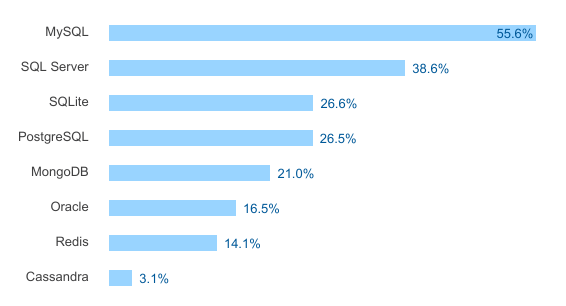
\includegraphics{dbstats.png}
\caption{Popularność rozwiązań DBMS, źródło: Stack Overflow Developer Survey 2017}
\label{fig:dbstats}
\end{figure}

      Bazy danych działające w pamięci RAM są wykorzystywane głównie podczas procesu wytwarzania oprogramowania, jako tymczasowe środowiska do testowania programów wymagających dowolnej bazy danych SQL. Typowe aplikacje, zwłaszcza internetowe, z reguły wymagają bazy danych, natomiast nie jest konieczne stosowanie tego samego rozwiązania przy tworzeniu oprogramowania, co przy wdrożeniu. Dzięki wykorzystaniu bibliotek typu ORM \cite{orm} (ang. \textit{Object Relational Mapping}) możliwe jest transparentne użycie dowolnej bazy, o ile aplikacja nie wykorzystuje specyficznych rozszerzeń języka SQL dostarczanych przez producentów. Powszechnie akceptowaną praktyką jest unikanie wiązania się z konkretną implementacją SQL. Dzięki wykorzystaniu pamięci programu jako miejsca zapisu danych, nie jest konieczne tworzenie baz poza aplikacją, a zawartość bazy czyszczona jest po zamknięciu programu. Interfejs programistyczny JDBC \cite{jdbc} jest wspierany przez wszystkie te rozwiązania, tak więc zarówno bazy dyskowe, jak i pamięciowe obsługuje się praktycznie w ten sam sposób. 

      Język SQL (ang. \textit{Structured Query Language}) jest językiem programowania przeznaczonym do interakcji z bazami danych, umożliwiającym odczyt, wstawianie i modyfikowanie zgromadzonych danych poprzez tekstowe polecenia. Został on opracowany na podstawie algebry relacji (Edgar F. Codd, 1970), wykorzystującej algebrę zbiorów jako podstawę teoretyczną. Jego niewątpliwą zaletą jest wykorzystanie do budowy zapytań prostych słów kluczowych w języku angielskim, które pozwalają na tworzenie bardzo czytelnych kodów. Duże możliwości zapewniają także bardziej zaawansowane elementy języka, takie jak funkcje agregujące czy zapytania wewnętrzne. Szczegóły na temat składni SQL znajdują się w \cite{ullman}, natomiast zestawienie sposobów konstruowania zapytań SQL i strumieniowych można znaleźć w rozdziale \ref{counterparts}.


\subsection{Stream API}

    Pojawienie się nowej wersji 8 platformy Java przyniosło dużo nowych zmian w języku. Wprowadzenie wyrażeń lambda jako zwięzłej alternatywy wobec anonimowych klas wewnętrznych, dodanie referencji do metod oraz wprowadzenie interfejsów domyślnych przełamało w pewien sposób popularną opinię, że język Java jest językiem jedynie obiektowym. Funkcyjne paradygmaty, coraz częściej analizowane i opisywane, okazują się dobrym sposobem na tworzenie bezpiecznych i łatwych w analizie aplikacji. Strumienie wykorzystują w bezpośredni sposób wszystkie powyższe, nowo wprowadzone udogodnienia. Skrócone funkcje lambda ułatwiają tworzenie prostych i silnie typowanych parametrów funkcyjnych, referencje do metod upraszczają pisanie odwzorowań operujących na aktualnie przetwarzanym obiekcie, a interfejsy domyślne pozwalają na tworzenie łatwiejszych w obsłudze interfejsów aplikacyjnych.

    Stream API jest komponentem biblioteki standardowej, który pozwala na tworzenie tzw. strumieni. Strumień jest abstrakcyjną reprezentacją ciągu obiektów, które pochodzą z pewnego źródła. Zazwyczaj strumienie tworzone są na podstawie kolekcji obiektów, ale ogólnie możliwe jest generowanie obiektów w dowolny sposób. Strumienie obsługują wykonywanie prostych i złożonych operacji filtrowania, sortowania, odwzorowania i grupowania, przy czym możliwe jest też samodzielne tworzenie obiektów przetwarzających dane (interfejs \texttt{Collector}). Należy mieć na uwadze, że wszystkie wykonane w ciągu operacje wykonywane są `leniwie', to znaczy żadna obróbka danych nie zachodzi przed wykonaniem tzw. operacji terminalnej. Wystąpienie operacji terminalnej powoduje łańcuchowe wykonanie się wszystkich operacji pośrednich.

    Cechą szczególną strumieni jest możliwość ich łatwego zrównoleglania, udostępniona programistom w postaci metody \texttt{Stream.parallelStream}. Wielowątkowe przetwarzanie danych jest dość złożonym zagadnieniem w Javie, wymagającym dużej wiedzy na temat działania maszyny wirtualnej (\textit{Java Memory Model}) i szczególnej ostrożności przy blokowaniu zasobów. Jako iż strumienie definiowane są zwykle przez funkcje nie zmieniające globalnego czy współdzielonego stanu, dodanie elementu równoległości jest znacznie prostsze. Jednym z celów niniejszej pracy jest zbadanie, jaki wpływ na wydajność mogą mieć równoległe strumienie.

\subsection{Przykład}

    Kod \ref{streamexample} prezentuje przykładowe użycie strumieni. Dostępna jest kolekcja \newline \texttt{Collection<Customer>}, która zawiera obiekty reprezentujące klientów. Każdy klient posiada pola danych, informujące między innymi o kraju jego pochodzenia oraz stanie konta (jest to część modelu danych TPC, który zostanie omówiony szczegółowo w rozdziale \ref{tpc}). Metoda \texttt{stream} tworzy strumień obiektów typu \texttt{Customer}, na którym wywoływane są metody strumieniowe. Metoda \texttt{filter} przyjmuje obiekt funkcyjny typu \texttt{Predicate}, który określa, czy dany element powinien znaleźć się w wynikowym strumieniu. Warto zaznaczyć, że możliwe jest wykorzystanie dowolnego kodu języka Java - nie ma tutaj ograniczeń na konkretny zbiór funkcji, jak w przypadku języka SQL. Metoda \texttt{sorted} zwraca nowy strumień, posortowany według podanego klucza - domyślnie porównywane są bezpośrednio obiekty znajdujące się w strumieniu. W tym przypadku wykorzystany został wariant metody sortującej, wykorzystujący funkcję wyłuskującą klucz sortowania z obiektu (tutaj - stan konta klienta). Na koniec wyniki zbierane są do listy typu \texttt{java.util.List}. 

\begin{lstlisting}[label=streamexample, caption=Przykładowe wykorzystanie Stream API]

List<Customer> canadiansSortedByBalance = 
customers.stream()
    .filter(customer -> Objects.equals(
        customer.nation.name,
        "CANADA"
    ))
    .sorted(Comparator.comparing(
        customer -> customer.acctbal
    ))
    .collect(toList());

\end{lstlisting}

\begin{figure}[h]
\centering
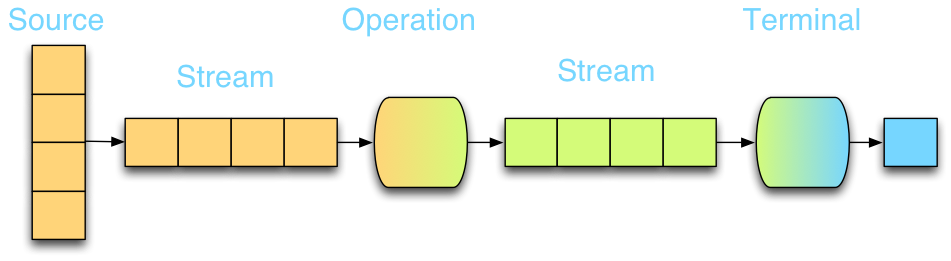
\includegraphics[width=14cm]{flow.png}
\caption{Przepływ danych}
\label{fig:flow}
\end{figure}

    Bardziej złożony przykład zaprezentowany jest w kodzie \ref{advanced}. Kolekcja zamówień, na której opiera się zapytanie, składa się z obiektów typu \texttt{Order} posiadająch status oraz przyporządkowanego do zamówienia klienta. Podobnie jak w przykładzie z kodu \ref{streamexample}, w pierwszym kroku przeprowadza się filtrowanie jedynie zamówień~o wyższym priorytecie. Następnie wykorzystana jest metoda \texttt{collect}, której zadaniem jest zebranie i przetworzenie danych w ostateczną postać wynikową. Wykorzystano tutaj dwa zagnieżdżone obiekty zbierające (ang. \textit{collectors}), z których pierwszy dokonuje grupowania zamówień na podstawie przypisanego klienta, a drugi odbiera pogrupowane zamówienia i dla każdej grupy określa ich wielkość, zliczając wszystkie obiekty w grupie. W ten sposób wyznaczone zostają liczby ważnych zamówień dla poszczególnych klientów.

\begin{lstlisting}[label=advanced, caption=Zaawansowane wykorzystanie Stream API]

List<String> high = asList("1-URGENT", "2-HIGH");
Map<Customer, Long> orderCountsByCustomer = orders
  .stream()
  .filter(o -> high.contains(o.orderPriority))
  .collect(
    Collectors.groupingBy(
      order -> order.customer,
      Collectors.counting()
    )
  );
  
    

\end{lstlisting}



\subsection{Interfejs \texttt{Collector}}

    Typ \texttt{Collector} jest ważną częścią Stream API. Pozwala on na definiowanie tzw. operacji terminalnych, czyli takich, które mogą występować jedynie na samym końcu potoku przetwarzania strumieniowego. Jest to dość niskopoziomowy mechanizm, który jednak nie jest zbyt skomplikowany, a wymusza na programiście zwrócenie uwagi na przetwarzanie równoległe. Parametrem wejściowym obiektu zbierającego jest strumień obiektów, przy czym nie jest on przekazywany jawnie, lecz poszczególne obiekty dostarczane są do odpowienich funkcji definujących obiekt zbierający. Wynikiem działania obiektu zbierającego jest obiekt lub kolekcja, będąca wynikiem operacji redukującej strumień danych. Instancja obiektu zbierającego nie posiada stanu - cały stan jest kontrolowany przez wewnętrzne struktury Stream API, co jest bardzo pożądane, zwłaszcza w przypadku strumieni równoległych, dla których zachowanie bezpieczeństwa wątkowego byłoby utrudnione.

    Do utworzenia obiektu \texttt{Collector} wymagane są trzy (w szczególnym przypadku cztery) funkcje:

\begin{itemize}
    \item \texttt{Supplier<T> supplier} - funkcja tworząca `pośredni zmienny kontener danych', będący tymczasową reprezentacją wyniku pośredniego,
    \item \texttt{BiConsumer<R, T> accumulator} - funkcja dodająca nowy element do pośredniego kontenera,
    \item \texttt{BinaryOperator<R> combiner} - funkcja scalająca dwa pośrednie kontenery w jeden,
    \item \texttt{Function<A, R> finisher} (opcjonalnie) - funkcja przekształcająca pośredni kontener danych w obiekt wynikowy.
\end{itemize}

    Konieczność istnienia pośrednich kontenerów i możliwości ich scalania związana jest bezpośrednio z równoległą naturą strumieni. Jako iż obiekty zbierające powinny działać w identyczny sposób ze strumieniami sekwencyjnymi, jak i równoległymi, narzucony został wzorzec uwzględniający przetwarzanie równoległe w każdym przypadku.

    Kod \ref{toList} prezentuje przykład ręcznie zaimplementowanego obiektu zbierającego \texttt{toList}, który dostępny jest domyślnie w bibliotece standardowej języka Java pod postacią metody statycznej \texttt{Collectors.toList}.

\begin{lstlisting}[label=toList, caption=Ręczna implementacja \texttt{toList}]

Collector<Integer, List<Integer>, List<Integer>> toList =
Collector.of(
    () -> {
      List<Integer> list = new ArrayList<>();
      out.println("New mutable container " + id(list));
      return list;
    },
    (acc, val) -> {
      out.println("Adding " + val + " to " + id(acc));
      acc.add(val);
    },
    (acc1, acc2) -> {
      out.println(
        "Combining " + id(acc1)
        + " with " + id(acc2)
      );
      acc1.addAll(acc2);
      return acc1;
    }
);

List<Integer> numbers = asList(1, 2, 3, 4, 5, 6, 7, 8, 9);

out.println(numbers.stream().collect(toList));

\end{lstlisting}

Wynik wykonania tego programu zaprezentowany jest na poniższym wyjściu. Warto zauważyć, że funkcja łącząca pośrednie kontenery nie została w~ogóle wywołana. 
    
\begin{verbatim}

New mutable container #6b7
Adding 1 to #6b7
Adding 2 to #6b7
Adding 3 to #6b7
Adding 4 to #6b7
Adding 5 to #6b7
Adding 6 to #6b7
Adding 7 to #6b7
Adding 8 to #6b7
Adding 9 to #6b7
[1, 2, 3, 4, 5, 6, 7, 8, 9]

\end{verbatim}

Przy wykorzystaniu strumieni równoległych, wynik prezentuje się zupełnie inaczej. Tworzona jest duża liczba kontenerów pośrednich, a wszystkie operacje dodawania i łączenia wykonywane są równolegle w osobnych wątkach.

\begin{verbatim}

New mutable container #42c
New mutable container #678
Adding 1 to #42c
New mutable container #2d8
New mutable container #1e6
New mutable container #1df
New mutable container #37c
New mutable container #585
New mutable container #51f
Adding 2 to #585
Adding 7 to #37c
Adding 3 to #1df
Adding 6 to #1e6
New mutable container #46f
Adding 4 to #2d8
Combining #1df with #2d8
Adding 5 to #46f
Adding 9 to #678
Combining #46f with #1e6
Combining #42c with #585
Adding 8 to #51f
Combining #42c with #1df
Combining #51f with #678
Combining #37c with #51f
Combining #46f with #37c
Combining #42c with #46f
[1, 2, 3, 4, 5, 6, 7, 8, 9]

\end{verbatim}

    Automatyczny podział pierwotnego zadania na zadania mniejsze, wykonanie ich, oraz ich późniejsze scalenie odbywa się w całości w wewnętrznym kodzie Stream API. Podany przykład jest przykładem znacznie uproszczonym. Możliwe jest wykonywanie bardzo złożonych operacji na danych (np. zbieranie statystyk), o ile możliwy jest podział i scalenie zadań.

\subsection{Biblioteka \texttt{ForkJoinPool}}

    Język Java od pierwszej wersji wyróżniał się znakomitymi możliwościami programowania równoległego, wykorzystywanego głównie w aplikacjach internetowych, obsługujących wielu użytkowników jednocześnie. Świadczy o tym obecność metod związanych z wątkami już w klasie \texttt{Object}, która jest klasą bazową wszystkich klas języka Java. W wersji 5 języka wprowadzono dużo nowych klas, zawartych w pakiecie \texttt{java.util.concurrent}, mających na celu ułatwienie pracy z kodem tego typu. Wcześniej ręcznie tworzone rozwiązania i wzorce mogą być zastąpione przez wbudowane, wysokiej jakości implementacje pul wątków, kolejek blokujących, list wykorzystującyc kopiowanie przy zapisie (\textit{copy-on-write}), semaforów i barier cyklicznych.
    
    Wersja siódma języka przyniosła kolejną nowość w postaci mechanizmu Fork-Join Pool \cite{fjpdocs}, umożliwiającego uproszczone tworzenie równolegle wykonywanych framentów kodu, wykorzystujące bezpośrednio regułę `dziel i zwyciężaj'. W programie wykorzystującym to rozwiązanie tworzona jest pula wątków (o dowolnej ilości), do której wysyła się zadanie, symbolizowane przez obiekt typu \texttt{RecursiveTask}. Klasa ta reprezentuje pojedyncze zadanie, które potrafi w razie potrzeby podzielić się na $ n $ mniejszych zadań. Kod programu powinien być w stanie zadecydować, czy zadanie jest zbyt duże czy i należy w związku z tym dokonać podziału. Jeśli tak, zadanie jest dzielone na podzadania i wysyłane do puli wątków, a po jego wykonaniu pośrednie wyniki zostają zebrane. Jeśli nie, program przystępuje do normalnego wykonywania przydzielonego zadania.  Przykładowy kod programu, mający na celu zsumowanie listy liczb całkowitych, zaprezentowany jest w kodzie \ref{fjpexample}.

\begin{lstlisting}[label=fjpexample, caption=Przykładowe wykorzystanie FJP]

public class SummingTask extends RecursiveTask<Integer> {
  
  private List<Integer> source;
  
  SummingTask(List<Integer> source) {
    this.source = source;
  }
  
  @Override
  protected Integer compute() {
    if (source.size() > 1) {
      List<SummingTask> tasks = splitTasks();
      
      invokeAll(tasks);
      
      int partialSum = 0;
      for (SummingTask task : tasks) {
        partialSum += task.join();
      }
      return partialSum;
    } else {
      return source.get(0);
    }
  }
  
  private List<SummingTask> splitTasks() {
    return asList(
        new SummingTask(source.subList(
          0, source.size() / 2)
        ),
        new SummingTask(source.subList(
          source.size() / 2, source.size()
        )
      )
    );
  }
  
  public static void main(String[] args) {
    ForkJoinPool forkJoinPool = new ForkJoinPool(10);
    SummingTask task = new SummingTask(
      asList(1, 2, 3, 4, 5, 6, 7, 8, 9)
    );
    Integer sum = forkJoinPool.submit(task).get();
    System.out.println(sum);
  }
}

\end{lstlisting}

\begin{figure}[h]
\centering
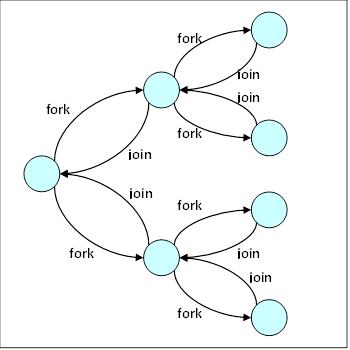
\includegraphics{forkjoin.png}
\caption{Wizualizacja działania mechanizmu Fork-Join (źródło: http://www.developer.com/imagesvr\_ce/3378/join-fork-image001.png)}
\label{fig:forkjoin}
\end{figure}


    FJP wykorzystany został przy implementacji równoległych strumieni. Jego znajomość nie jest konieczna do ich używania, natomiast może być przydatna przy badaniu wydajności przetwarzania strumieniowego. Domyślnie, przy tworzeniu strumienia nie jest możliwe wybranie puli wątków, w której przetwarzanie będzie zachodzić - przy bezpośrednim użyciu FJP jest to możliwe (metoda \texttt{submit}), wraz z określeniem docelowej, maksymalnej liczby wątków. Przeprowadzono dodatkowy eksperyment, w którym zbadano wydajność (liczbę operacji na sekundę) sortowania 1000000 liczb całkowitych, przy wykorzystaniu równoległych strumieni i zadania wykonywanego bezpośrednio w puli FJP, w zależności od liczby wątków puli. Kod źródłowy znajduje się w pliku \texttt{FJPSorting.java}, a rysunek \ref{fig:fjpsorting} prezentuje wyniki eksperymentu.

\begin{figure}[H]
\centering
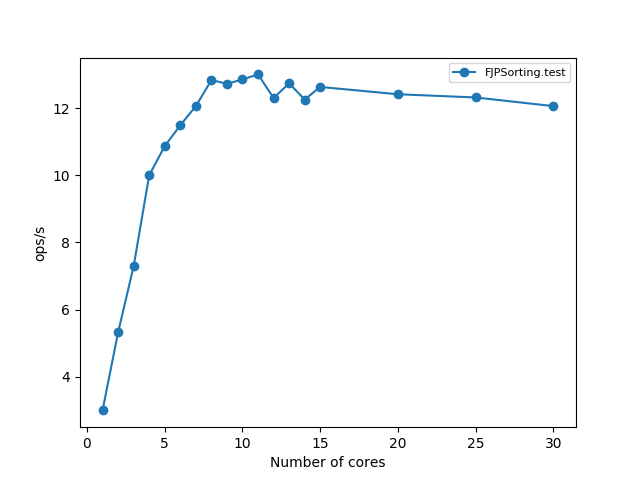
\includegraphics[width=13cm]{plots/FJPSorting}
\caption{Sortowanie 1000000 liczb w puli wątków FJP}
\label{fig:fjpsorting}
\end{figure}

    Jak można zauważyć, liczba operacji na sekundę rośnie przy wzroście wielkości puli do pewnego momentu, w którym narzut tworzenia i wykorzystywania nowych wątków staje się zbyt duży. Przyjęło się za ogólnie dobrą praktykę, aby liczba wątków była w przybliżeniu równa liczbie logicznych rdzeni procesora, ponieważ umożliwia to najlepsze wykorzystanie mocy obliczeniowej. Test przeprowadzono na maszynie z 4 rdzeniami Hyper Threading (logiczne 8 rdzeni), w związku z tym można się spodziewać największej liczby operacji na sekundę dla mniej więcej 8 wątków.


\subsection{Przetwarzanie równoległe}

    Jednym z najczęstszych zastosowań strumieni jest równoległe przetwarzanie danych. Strumienie równoległe wykorzystują FJP, natomiast w pełni ukrywają fakt jego użycia w taki sposób, że w większości przypadków wiedza na temat szczegółów implementacyjnych nie jest konieczna. Poszczególne zadania przetwarzania danych (filtrowanie, odwzorowanie itd.) wykonują się w tworzonej przy starcie maszyny wirtualnej puli wątków, w której domyślnie znajduje się $ n-1 $ wątków, gdzie $ n $ jest liczbą logicznych rdzeni procesora. Najlepiej widać to w kodzie \ref{streamsthreads}, w którym dla każdego elementu wypisywana jest nazwa wątku, w którym kod funkcji jest wykonywany.  Wynikiem wywołania tego programu jest przemieszana lista wątków, w której znajdują się wątek główny programu \texttt{main} oraz wątki znajdujące się w puli o nazwach \texttt{ForkJoinPool.commonPool-worker-N} z numerami od 1 do 7 (test przeprowadzony na maszynie z 8 logicznymi procesorami).

\begin{lstlisting}[label=streamsthreads, caption=Struktura puli wątków FJP]

IntStream.range(1, 100).parallel()
  .forEach(e -> out.println(
    Thread.currentThread().getName()
  )
);

\end{lstlisting}

\begin{verbatim}
...
ForkJoinPool.commonPool-worker-1
ForkJoinPool.commonPool-worker-4
ForkJoinPool.commonPool-worker-4
ForkJoinPool.commonPool-worker-7
ForkJoinPool.commonPool-worker-7
ForkJoinPool.commonPool-worker-7
ForkJoinPool.commonPool-worker-6
ForkJoinPool.commonPool-worker-6
ForkJoinPool.commonPool-worker-6
ForkJoinPool.commonPool-worker-2
ForkJoinPool.commonPool-worker-3
ForkJoinPool.commonPool-worker-3
ForkJoinPool.commonPool-worker-3
ForkJoinPool.commonPool-worker-5
main
main
...
\end{verbatim}

    Warto zwrócić uwagę, że wśród wątków wykonawczych znajduje się też wątek \texttt{main}, czyli wątek inicjujący operację strumieniową. Jako iż wykonywanie się ciągu operacji strumieniowych jest blokujące (nie jest asynchroniczne, o ile nie wykorzystuje się FJP ręcznie), dobrym rozwiązaniem jest wykorzystanie do obliczeń także wątku inicjującego. Jeśli nie jest to oczekiwane zachowanie, istnieje możliwość ręcznego utworzenia instancji puli wątków \texttt{ForkJoinPool} i przekazanie zadania w~postaci funkcji lambda \texttt{Callable<T>}. W takim podejściu możliwe jest też zdefiniowanie liczby dostępnych wątków.

\cleardoublepage
\section{Porównanie przetwarzania strumieniowego i zapytań SQL}

    Pomiędzy wykonywaniem operacji strumieniowych, a wykonywaniem zapytań SQL w pamięci występuje bardzo dużo różnic, zwłaszcza w zakresie konstruowania zapytań i sposobu ich realizacji, pomimo pozornie podobnej zasady działania i efektu końcowego. Celem obu podejść jest uzyskanie wygodnego i względnie szybkiego wykonywania zapytań, natomiast różnice w implementacji mają znaczący wpływ na te kwestie.

\subsection{Struktury danych}

    Głównym blokiem budującym w modelu relacyjnej bazy danych jest relacja (tabela) posiadająca kolumny i rekordy, a integralność danych zapewniona jest w pewnym stopniu przez ograniczenia, klucze i więzy referencyjne. Język SQL pozwala dzięki mechanizmowi JOIN na łatwe łączenie powiązanych ze sobą tabel i uzyskiwanie połączonych wyników. Jeśli baza danych została odpowienio zaprojektowana, uwzględniając normalizację danych, to łączenie tabel na podstawie kluczy obcych jest naturalne dla programisty i proste w zrozumieniu. W przetwarzaniu strumieniowym pojęcie tabeli nie istnieje, ponieważ kontenerami danych są zwykłe kolekcje języka Java (listy, zbiory i mapy). O ile istnieją biblioteki bazodanowe typu jOOQ, które pozwalają na konwersję wyniku zapytania JDBC na strumień, to tak naprawdę operacje strumieniowe wykonują się zawsze na kolekcji w pamięci maszyny wirtualnej. W konsekwencji, aby operacje strumieniowe były wygodne dla programisty, model danych powinien uwzględniać powiązania między poszczególnymi obiektami w typowy dla języka Java sposób, poprzez referencje do innych obiektów (kompozycja). Łączenie kolekcji, choć możliwe, komplikuje znacznie zapytania i zmniejsza ich ogólną szybkość.

\begin{figure}[h]
\centering
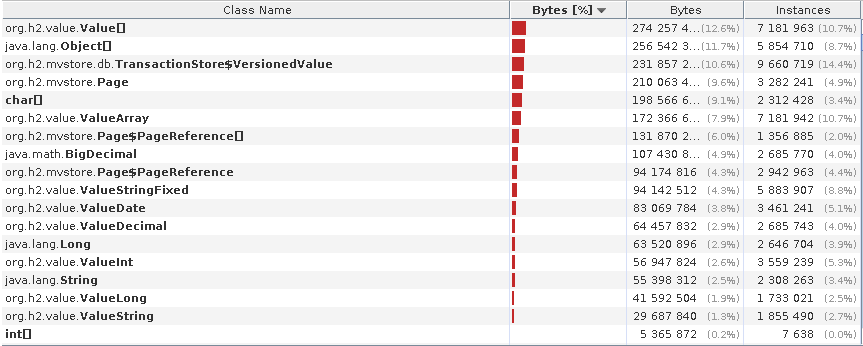
\includegraphics[width=15cm]{jvmmemory}
\caption{Migawka statystyk wykorzystania pamięci maszyny wirtualnej (narzędzie VisualVM)}
\label{fig:jvmmemory}
\end{figure}

    Bazy pamięciowe wykorzystują wewnętrzne struktury danych, które są ścisłym szczegółem implementacyjnym, niewidocznym dla programisty i zabezpieczonym przed zmianami. Jest to w większości przypadków dobre rozwiązanie, pozwalające na odseparowanie wewnętrznej reprezentacji danych od metody dostępu do nich (przykładowo, dane w bazie H2 reprezentowane są przez obiekty klas implementacyjnych z pakietu \texttt{org.h2.*} - rysunek \ref{fig:jvmmemory}). Jednakże przy takim podejściu programista nie ma możliwości optymalizacji (o ile to możliwe) struktur danych i musi polegać na wykorzystanym w silniku bazy optymalizatorze zapytań. W przypadku strumieni wewnętrzne procesy zachodzące przy przetwarzaniu danych są ukryte, natomiast możliwe jest w każdym przypadku przepisanie części procesu na czystą Javę. Strumienie są bardzo wydajne, natomiast tak jak każda abstrakcja nad danymi wprowadzają pewnien niewielki narzut. W przypadku, gdy szybkość jest parametrem krytycznym, możliwe jest zastąpienie operacji klasy \texttt{Stream} zwykłymi konstrukcjami języka (pętle, warunki). 

\subsection{Język dziedzinowy a język ogólnego przeznaczenia}

    Język SQL, poza metodami dostępu do danych umożliwia także ich wstępne przetwarzanie. Dostępne są proste funkcje matematyczne, funkcje operujące na ciągach znaków czy datach. Problemem jest jednak często brak standaryzacji - różni dostawcy baz danych rozszerzają możliwości języka o różne funkcje, przez co migracja pomiędzy bazami danych może być problematyczna, zwłaszcza, jeśli w użyciu są własne procedury składowane (ang. \textit{stored procedures}). 
   
    Przy użyciu Stream API możliwe jest wykorzystanie praktycznie dowolnego kodu Javy, przez co aplikacja je wykorzystująca jest znacznie bardziej przenośna i łatwiej testowalna. Przykładem jest obsługa dat - język Java wyposażony został w wersji 8 w klasy pakietu \texttt{java.time.*}, umożliwiające wygodne i poprawne operacje na datach i interwałach czasowych, przy uwzględnieniu stref czasowych. Funkcje SQL są ograniczone w~tym zakresie i ich rozszerzanie nie jest zbyt wygodne.

    Za przykład niech posłuży zadanie znalezienia daty pierwszego poniedziałku aktualnego miesiąca. Takie problemy pojawiają się często przy tworzeniu różnych statystyk na podstawie danych historycznych. W kodzie \ref{date} zaprezentowany jest przykład rozwiązania powyższego problemu, odpowiednio przy użyciu MySQL i Stream API.
    

\begin{lstlisting}[label=date, caption=Problem znalezienia pierwszego poniedziałku w miesiącu]
set @firstday = DATE_ADD(
  LAST_DAY(
    DATE_SUB(CURDATE(), interval 30 day)
  ),
  interval 1 day
);
SELECT ADDDATE(
  @firstday,
  MOD((9 - DAYOFWEEK(@firstday)), 7))
as first_monday;


LocalDateTime.now()
  .with(dayOfWeekInMonth(1, DayOfWeek.MONDAY));
\end{lstlisting}

Można od razu zauważyć, że kod SQL jest dość nieczytelny i zawiera wiele szczegółów technicznych, które nie są istotne dla postawionego problemu. Wprowadzone w Java 8 nowe mechanizmy obsługi dat sprawdzają się w takich przypadkach znacznie lepiej, zapewniając bardzo deklaratywny kod i bezpieczne, statyczne typowanie.


\subsection{Odpowiedniki operacji} \label{counterparts}

    Stream API umożliwia wykonywanie wielu operacji znanych z języka SQL. Część z nich posiada dokładne odpowiedniki (np. ograniczanie ilości czy filtrowanie), natomiast niektóre wymagają częściowo ręcznej implementacji (złączenie albo unia). Należy zauważyć, iż mimo istnienia pewnej wspólnej bazy pojęciowej, sposób przekazywania parametrów do operacji może być zupełnie inny. Przykładowo, aby wykonać sortowanie w SQL na podstawie kilku kolumn, wystarczy wymienić klucze sortowania po przecinku, przykładowo w postaci \texttt{ORDER BY col1, col2}. Silnik bazodanowy jest w stanie wewnętrznie zinterpretować takie zapytanie. Do sortowania strumieni konieczne jest uzyskanie obiektu typu \texttt{Comparator}, który przekazany zostanie do metody sortującej, a utworzyć można go np. poprzez \texttt{Comparator.comparing(e -> e.col1).thenComparing(e -> e.col2)}. Obiekt taki jest całkowicie odseparowany od strumienia i może być tworzony w dowolnym miejscu w kodzie.

\begin{table}[t]
    \label{nazwa odnośnika, która potem użyjemy do cytowania tabeli}
    \begin{center}
        \begin{tabular}{ |c|c| }
            \hline
            \textbf{SQL} & \textbf{Stream API} \\
            \hline
            \texttt{SELECT} & \texttt{.map(...)}  \\
            \texttt{FROM} & \texttt{.stream()}  \\
            \texttt{WHERE} & \texttt{.filter(...)}  \\
            \texttt{JOIN ON} & \texttt{.flatMap(...).filter(...)}  \\
            \texttt{HAVING} & \texttt{.filter(...)}  \\
            \hline
            \texttt{DISTINCT} & \texttt{.distinct()}  \\ 
            \texttt{UNION ALL} & \texttt{Stream.concat(..., ...)} \\
            \texttt{UNION} & \texttt{Stream.concat(..., ...).distinct()}  \\
            \hline
            \texttt{ORDER BY} & \texttt{.sorted(...)}  \\
            \texttt{LIMIT} & \texttt{.limit(...)}  \\
            \texttt{OFFSET} & \texttt{.skip(...)}  \\
            \hline
        \end{tabular}

        \caption{Odpowiedniki operacji w języku SQL i Stream API}
    \end{center}
\end{table}

\subsection{Strumieniowy operator złączenia} \label{proposal}

    Jedną z najczęściej wykonywanych operacji na relacyjnej bazie danych jest łączenie tabel. W języku SQL dostępne są różne typy złączeń (\texttt{JOIN}, \texttt{INNER JOIN}, \texttt{LEFT/RIGHT JOIN} i inne), które wykorzystywane są w różnych sytuacjach. Relacyjne bazy danych posiadają z reguły znaczne optymalizacje w zakresie wykonywania takich operacji, ponieważ wykorzystywane są one bardzo często - ważną zaletą modelu relacyjnego jest podział na tabele połączone ze sobą kluczami i więzami referencyjnymi. Aby osiągnąć wymaganą wydajność, w większości rozwiązań kolumny będące kluczami głównymi otrzymują automatycznie, przy ich tworzeniu, indeks.

    Indeks jest strukturą danych, zbudowaną na podstawie wartości danych określonej kolumny (kolumn) danej tabeli. Bazuje on zwykle na drzewiastej strukturze danych, gromadzącej wszystkie pary klucz-wartość z indeksowanej kolumny, gdzie kluczem jest zawartość kolumny, a wartością wskaźnik do wiersza, zawierającego daną wartość. Dzięki ustanowionemu porządkowi (drzewo jest posortowane) i korzystnych złożonościach wyszukiwania, możliwe jest zastąpienie liniowego wyszukiwania w liście szybkim wyszukiwaniem w drzewie. Bazy danych SQL bardzo często wykorzystują indeksy, większość z nich tworzy domyślnie indeks na kolumnach będących kluczami głównymi nowo dodawanej tabeli. Wydaje się więc wskazane, aby wypróbować podobne rozwiązanie w przypadku łączenia strumieni. Jako kontener danych wykorzystano implementację zbioru mieszającego z biblioteki standardowej języka Java, \texttt{java.util.HashSet}, ze względu na jego wydajność. Istnieje też alternatywne rozwiązanie w postaci kontenera \texttt{java.util.TreeSet} wykorzystującego zmodyfikowane drzewo czerwono-czarne, natomiast jest ono mniej wydajne niż rozwiązanie z kolekcją mieszającą.

    Ze względu na porównawczy charakter niniejszej pracy, zdecydowano się na opracowanie podobnego rozwiązania, działającego w oparciu o Stream API. Problem zdefiniowany został następująco:

\begin{theorem}
    Dane są dwie kolekcje typów \texttt{T} i \texttt{U} o rozmiarach $ n $ i $ m $. Należy zaproponować rozwiązanie, pozwalające na złączenie tych kolekcji na podstawie warunku równości dowolnych kluczy, będących właściwościami obiektów, bądź funkcjami właściwości obiektów. Wynik powinien dany być listą par \texttt{(T, U)}.
\end{theorem}

    Pierwsze rozwiązanie, najbardziej intuicyjne, polega utworzeniu wszystkich możliwych par \texttt{(T, U)} i wyfiltrowaniu pożądanych. Do tego celu wykorzystano metodę \texttt{Stream.flatMap}, która dla każdego obiektu strumienia tworzy nowy strumień nań bazujący, a następnie łączy wszystkie pośrednie strumienie w jeden.

\begin{lstlisting}[label=join1, caption=Rozwiązanie nr 1]
public static <T, U> Stream<ImmutablePair<T, U>>
innerJoin(
    Collection<T> first,
    Collection<U> second,
    Predicate<ImmutablePair<T, U>> condition
) {
  return first.stream().flatMap(firstItem ->
      second.stream().map(secondItem ->
          new ImmutablePair<>(firstItem, secondItem)
      )
  ).filter(condition);
}

\end{lstlisting}

    Rozwiązanie to, mimo iż krótkie i czytelne, wykazuje się bardzo niekorzystną złożonością obliczeniową, i w konsekwencji, bardzo słabą wydajnością. Ze względu na konieczność utworzenia $ mn $ par niezależnie od przypadku, aktywność GC jest znaczna, ponieważ mnóstwo obiektów tworzonych jest tylko w celu ich odśmiecenia. Przykładowo, dla współczynnika wielkości zbioru TPC wynoszącego 20\% połączenie tabeli \texttt{Orders} (300000 wierszy) i \texttt{Lineitem} (1119969 wierszy) powoduje wygenerowanie około 350 miliardów obiektów.

    Rozwiązanie drugie polega na przepisaniu strumieniowej części w postaci zwykłej pętli. Strumienie mają nieznaczny narzut czasowy i pamięciowy, więc warto sprawdzić, czy możliwe jest jego uniknięcie.

\begin{lstlisting}[label=join2, caption=Rozwiązanie nr 2]

public static <T, U> Stream<ImmutablePair<T, U>>
innerJoinForLoop(
    Collection<T> first,
    Collection<U> second,
    BiPredicate<T, U> condition
) {
  List<ImmutablePair<T, U>> result = new ArrayList<>();
  for (T t : first) {
    for (U u : second) {
      if (condition.test(t, u)) {
        result.add(new ImmutablePair<>(t, u));
      }
    }
  }
  return result.stream();
    

\end{lstlisting}

    To rozwiązanie jest nieco lepsze, natomiast nie jest znacząco lepsze od poprzedniego. Problemem jest konieczność przejścia przez wewnętrzną pętlę nadal $ mn $ razy.

    W rozwiązaniu trzecim postanowiono wykorzystać kolekcje mieszające, które spełniają w nim rolę podobną do indeksów. Przy założeniu, że kolekcje łączone są warunkiem równości właściwości, z których co najmniej jedna spełnia właściwości klucza głównego (unikalność i brak występowania wartości pustej \texttt{NULL}), możliwe jest umieszczenie elementów tej kolekcji w strukturze mapy mieszającej, w której za klucz przyjmuje się wymieniony klucz główny, a za wartość - obiekt przez ten klucz reprezentowany. Dzięki temu, nie jest wymagane przeglądanie całej kolekcji elementów \texttt{T}, a jedynie sprawdzenie, czy obiekt identyfikowany przez kolejne obiekty kolekcji \texttt{U} istnieje bądź nie.

\begin{lstlisting}[label=join3, caption=Rozwiązanie nr 3]

public static <T, U> Stream<ImmutablePair<T, U>> 
innerJoinHashmaps(
    Collection<T> left,
    Function<T, Object> leftKeyExtractor,
    Collection<U> right,
    Function<U, Object> rightKeyExtractor
) {
  HashMap<Object, T> leftMap = new HashMap<>();
  for (T leftElement : left) {
    leftMap.put(
      leftKeyExtractor.apply(leftElement),
      leftElement
    );
  }
  
  List<ImmutablePair<T, U>> result = new ArrayList<>();
  
  for (U rightElement : right) {
    T leftElement = leftMap.get(
      rightKeyExtractor.apply(rightElement)
    );
    if (leftElement != null) {
      result.add(new ImmutablePair<>(
        leftElement, rightElement
      ));
    }
  }
  
  return result.stream();
}
\end{lstlisting}

Rozwiązanie to jest znacznie szybsze, wymaga jednak unikalności wartości klucza w jednej z kolekcji. Porównanie szybkości wykonywania się operacji złączenia na zbiorze danych TPC zaprezentowane jest w rozdziale \ref{tpcgraphs} na rysunku \ref{fig:naturaljoingraph}.


\subsection{Proces wykonywania zapytania SQL}

    Jedną z ważniejszych cech języka programowania jest sposób interpretacji kodu programu przez interpreter bądź kompilator. Język SQL wykazuje szczególne zachowanie, ponieważ leksykalna kolejność operacji jest odmienna od logicznej kolejności. Kod \ref{sqlexample} prezentuje przykładowe zapytanie SQL, przeznaczone do wykonania na testowej bazie TPC:


\begin{lstlisting}[label=sqlexample, caption=Przykład kolejności wykonywania zapytania SQL]
select customers.name, sum(order.totalprice)
from orders 
    join customers on customers.custkey = orders.custkey
where customer.acctbal > 1000
group by customers.custkey, customers.name
having sum(order.totalprice) > 10000
order by customers.name;
\end{lstlisting}

    Bazy SQL posiadają zwykle optymalizatory zapytań o różnym stopniu złożoności. Możliwe jest sprawdzenie dokładnego planu zapytania (ang. \textit{query execution plan}) za pomocą składni odpowiedniej dla danego systemu, przykładowo, w MySQL istnieje specjalna klauzula \texttt{EXPLAIN}. Optymalizacje i zmiany kolejności nie wpływają jednak na wynik, który jest zawsze taki sam, jak przy wykonywaniu zapytania zgodnie z logiczną kolejnością SQL. Zapytanie zamieszczone we fragmencie \ref{sqlexample} posiada następującą kolejność wykonywania:

\begin{itemize}
    \item \textbf{from orders join customer} - wybranie tabeli (tabel), z których pobrane zostaną dane (należy zaznaczyć, że klauzula \textbf{join} jest logicznie częścią klauzuli \textbf{where}, jedynie skrótowo zapisaną),
    \item \textbf{where customer.acctbal > 1000} - filtrowanie wierszy, odrzucenie niechcianych danych,
    \item \textbf{group by customers.custkey, customers.name} - tworzenie grup na podstawie podanej krotki, podczas grupowania obliczane są wszystkie funkcje agregujące występujące w zapytaniu,
    \item \textbf{having sum(order.totalprice) > 10000} - filtrowanie całych grup, na podstawie wyliczonych w poprzednim kroku funkcji (tutaj sprawdzana jest wartość sumy),
    \item \textbf{select customers.name, sum(order.totalprice)} - wybranie, na podstawie pośredniej tabeli zawierającej jak dotąd wszystkie kolumny z obu tabel (po połączeniu), jedynie wymaganych kolumn,
    \item \textbf{order by customers.name} - sortowanie według jednej lub kilku wybranych kolumn.
\end{itemize}

    Jak można zauważyć, logiczna kolejność wykonywania zapytania jest znacząco odmienna od faktycznej kolejności. Wynikiem zapytania jest zbiór wierszy (krotek) z dwoma kolumnami, odpowiednio typu znakowego oraz liczbowego.

\subsection{Proces wykonywania zapytania strumieniowego}

    Podobnie jak w przypadku języka SQL, zapytanie strumieniowe wykonuje się w~kilku etapach. Ważną różnicą jest to, że nie występuje tutaj żaden mechanizm parsowania i tłumaczenia kodu, ponieważ zwykły kod języka Java jest już skompilowany do kodu bajtowego i wykonywany na maszynie wirtualnej. Maszyna wirtualna po uruchomieniu programu realizuje dużą liczbę optymalizacji kodu, więc możliwe jest uzyskanie wzrostu wydajności także dzięki tym optymalizacjom. Kod \ref{streamsexample} przezentuje zapytanie strumieniowe odpowiadające zapytaniu z kodu \ref{sqlexample}:

\begin{lstlisting}[label=streamsexample, caption=Analogiczne rozwiązanie wykorzystujące Stream API]
List<Pair<String, Double>> result = StreamUtils.innerJoin(
    store.getOrders(),
    store.getCustomers(),
    pair -> pair.left.customer.equals(pair.right)
)
    .filter(pair ->
        pair.right.acctbal.doubleValue() > 1000
    )
    .collect(groupingBy(
        pair -> new ImmutablePair<>(
            pair.right.custkey,
            pair.right.name
        ),
        summingDouble(pair ->
            pair.left.totalPrice.doubleValue()
        ))
    )
    .entrySet().stream()
    .filter(entry -> entry.getValue() > 10000)
    .map(entry -> new ImmutablePair<>(
        entry.getKey().right,
        entry.getValue()
    ))
    .collect(toList());
\end{lstlisting}

    Pod względem liczby linii kodu oraz czytelności przykład ten prezentuje się mniej korzystnie. W celu wyrażenia tego samego zapytania w Stream API konieczne jest wykorzystanie kilku ręcznych mechanizmów. Strumienie nie wspierają złączeń kolekcji, tak więc konieczne jest ręczne jego wykonanie (propozycja implementacji znajduje się w rozdziale \ref{proposal}). Wynikiem złączenia jest lista par, na której odbywa się filtrowanie, a następnie grupowanie. Aby pogrupować elementy strumienia na podstawie kilku właściwości, konieczne jest ponowne użycie klasy \texttt{ImmutablePair<T1, T2>}, której obiekty reprezentują klucz mapy, na podstawie którego odbywa się grupowanie. Jako iż klasa \texttt{Map} nie udostępnia bezpośrednio możliwości tworzenia strumieni, konieczne jest wykorzystanie metody \texttt{Map.entrySet} w celu uzyskania zbioru par klucz-wartość, na którym ponownie wywoływana jest metoda tworząca strumień. Na koniec z utworzonych grup wyłuskiwane są wymagane pola (imię klienta oraz suma cen zamówień) i zbierane do listy.

    Strumień, będąc abstrakcyjną formą reprezentacji źródła danych, tworzony może być na kilka różnych sposobów, ale sposoby te nie wpływają semantycznie na proces przetwarzania danych. Zwykle strumień tworzony jest na podstawie kolekcji - przy konsumowaniu elementów, kolekcja dostarcza elementy wykonując wewnętrzną iterację (\textit{internal iteration}), która jest procesem ukrytym przed programistą. Inne sposoby tworzenia strumieni, takie jak generowanie ich w locie, wczytywanie z dysku bądź z sieci, nie są zbyt praktyczne. Związane jest to z konstrukcją wewnętrzną strumieni, które działają na zasadzie `pytania o kolejny element` (\textit{pull-based}). Decyzją implementacyjną projektantów Stream API było wykorzystanie modelu przetwarzania ciągłego, w którym to strumień wykonuje akcję pobrania następnego elementu. W~związku z tym, nie jest możliwe (przynajmniej w domyślnej formie) efektywne asynchroniczne dostarczanie nowych elementów, ponieważ każda operacja pobrania elementu jest operacją blokującą, wywoływaną po zakończeniu przetwarzania poprzedniego elementu. Model odwrotny do powyższego, tzw. model \textit{push-based}, wykorzystywany np. w bibliotekach RxJava bazujących na wzorcu Observable, ma lepsze zastosowanie w takich przypadkach. Brian Goetz, zapytany o możliwości przetwarzania asynchronicznego w domyślnych strumieniach Java 8 stwierdził:

\begin{quote}
    ``The design center for Streams is mostly about data that can be accessed with no latency (either from data structures or generating functions); the design center for Rx is about infinite streams of events which may arrive asynchronously \cite{goetz}''

    ``Zamiarem architektonicznym Stream API było przetwarzanie danych, które są dostępne bez żadnych opóźnień (pochodzących ze struktur danych bądź funkcji generujących), celem Rx jest obsługa nieskończonych strumieni zdarzeń, które mogą pojawiać się asynchronicznie''
    (\textit{tłumaczenie autora})

\end{quote}


    Po utworzeniu strumienia możliwe jest wykonanie dostępnych na nim operacji pośrednich, udostępnionych przez metody instancyjne klasy \texttt{Stream<T>}. Każda taka operacja zwraca zawsze strumień, ewentualnie innego typu (\texttt{Stream<...>}, \texttt{IntStream}). Należy zwrócić szczególną uwagę na różnice pomiędzy dwoma typami operacji pośrednich, ponieważ owe typy determinują faktyczną, wewnętrzną kolejność operacji, która mimo iż ukryta przed programistą, może mieć wpływ na złożoność czasową jak i pamięciową. Operacje pośrednie bezstanowe (takie jak \texttt{filter} i \texttt{map}) zapisane tuż obok siebie, łączone są w jedną, większą operację, wykorzystując właściwości kompozycji funkcji bezstanowych. Drugi typ operacji pośrednich, operacje pośrednie stanowe, nie gwarantują fuzji i mogą wprowadzać ukryty stan. Najlepszym przykładem operacji pośredniej stanowej jest sortowanie, które wymaga, aby dokładnie wszystkie elementy strumienia zbuforowane zostały przed sortowaniem. Jest to logiczne, ponieważ nie jest możliwe ustalenie posortowanej kolejności zbioru elementów o nieznanej wielkości. Przykład fuzji operacji zaprezentowany jest w kodzie \ref{streamstateful1}.

\begin{lstlisting}[label=streamstateful1, caption=Fuzja operacji bezstanowych]
Stream.of(1, 2, 3, 4, 5)
    .map(e -> {
      out.println("Mapping: " + e);
      return e;
    })
    .filter(e -> {
      out.println("Filtering: " + e);
      return true;
    })
    .sorted()
    .collect(toList());

\end{lstlisting}


\begin{verbatim}

Mapping: 1
Filtering: 1
Mapping: 2
Filtering: 2
Mapping: 3
Filtering: 3
Mapping: 4
Filtering: 4
Mapping: 5
Filtering: 5

\end{verbatim}

    Na podstawie wyjścia programu można stwierdzić, że operacja \texttt{map} wykonywała się wraz z operacją \texttt{filter}. Jako iż sortowanie zostało umieszczone na końcu, nie przeszkadzało ono w żaden sposób. Z drugiej strony, jeśli sortowanie zostanie przeniesione pomiędzy, można zaobserwować buforowanie się elementów tuż przed stanową operacją sortowania (fragment \ref{streamstateful2}).

\begin{lstlisting}[label=streamstateful2, caption=Brak fuzji operacji stanowych]
Stream.of(1, 2, 3, 4, 5)
    .map(e -> {
      out.println("Mapping: " + e);
      return e;
    })
    .sorted()
    .filter(e -> {
      out.println("Filtering: " + e);
      return true;
    })
    .collect(toList());
\end{lstlisting}

\begin{verbatim}

Mapping: 1
Mapping: 2
Mapping: 3
Mapping: 4
Mapping: 5
Filtering: 1
Filtering: 2
Filtering: 3
Filtering: 4
Filtering: 5

\end{verbatim}

    Ostatnim krokiem wykonywania się zapytania strumieniowego jest wykonanie operacji terminalnej, która wyznacza ostateczny wynik zapytania. Wystąpienie takiej operacji powoduje wykonanie wszystkich operacji pośrednich. 

\subsection{Weryfikacja poprawności składni i postać wyników zapytania}

    Przy wykonywaniu zapytania SQL z poziomu API JDBC nie jest wykonywane żadne sprawdzenie poprawności zapytania czy jego składni w czasie kompilacji. Zapytanie wysyłane jest jako zwykły ciąg znaków do serwera bazodanowego, który następnie odczytuje zapytanie, przystępując do jego interpretacji i wykonania. W związku z tym niemożliwe jest zapewnienie, czy dana tabela istnieje, albo czy dana funkcja SQL istnieje w danym oprogramowaniu bazy danych. Istnieją co prawda rozwiązania typu ORM, które chronią programistę przed niewłaściwym wykorzystaniem obiektu odwzorowanego na tabelę, albo edytory programistyczne z integracjami z serwerami baz, które umożliwiają przeskanowanie istniejących symboli (nazw tabel, kolumn itp.) i skorygowanie programisty, natomiast są to rozwiązania zewnętrzne, działające poza językiem Java. Przetwarzanie strumieniowe odbywa się w całości w języku Java, który jest silnie typowany, przez co niewłaściwe wykorzystanie konstrukcji języka zostanie automatycznie dostrzeżone przez kompilator.
    
    Jako przykład dobrana została sygnatura statycznej metody \newline \texttt{Collectors.groupingBy}, zaprezentowana we fragmencie \ref{genericsexample}. Dzięki zastosowaniu typów ogólnych \cite{generics} (generycznych), możliwe jest zagwarantowanie zgodności typów, o ile nie zostanie zastosowanie niebezpieczne rzutowanie.

\begin{lstlisting}[label=genericsexample, caption=Sygnatura metody grupującej]
  public static <T, K> Collector<T, ?, Map<K, List<T>>>
  groupingBy(Function<? super T, ? extends K> classifier) 
  { ...  }
\end{lstlisting}

    Przykładowo, wynikiem grupowania zbioru obiektów typu \texttt{T} (bądź jego typu pochodnego) na podstawie ich pola o typie \texttt{K} (bądź pola typu dziedziczonego) będzie zawsze \texttt{Map<K, List<T>}\texttt{>}. Dzięki temu typowe błędy przy odczytywaniu wyników z zapytania SQL przy użyciu obiektu \texttt{ResultSet} (niewłaściwy typ kolumny, niestniejące pole) nie występują.

    Wynikiem poprawnego zapytania SQL jest zawsze lista krotek, zawierająca wszystkie wiersze pasujące do zapytania i wszystkie kolumny wymienione w klauzuli \texttt{SELECT}. Przy wykonywaniu zapytania z poziomu silnie typowanego języka programowania obiekt reprezentujący wynik zapytania nie posiada informacji o typach danych kolumn. Przykładowo, w języku Java, do wyciągania danych służą obiekty klasy \texttt{ResultSet} udostępniające metody typu \texttt{getInt} czy \texttt{getString}. Błąd programisty polegający na użyciu niewłaściwej metody zakończy się wyjątkiem w czasie działania programu i nie jest możliwy do automatycznego wykrycia przed próbą uruchomienia programu. W przypadku Stream API, wynikiem zapytania jest zawsze typ języka Java, a poprawność syntaktyczna gwarantowana jest przez kompilator i złożony system typów języka. Próba odwołania się do nieistniejącego pola bądź próba wykonania niewłaściwej operacji na określonym typie danych nie skompiluje się. 

\subsection{Podsumowanie}

    Wprowadzenie do języka Java mechanizmów programowania funkcyjnego zostało bardzo pozytywnie ocenione przez programistów, mimo iż mechanizmy te obecne były w innych językach programowania ogólnego przeznaczenia znacznie wcześniej. Duży nacisk projektantów platformy na wsteczną kompatybilność i obawy przed wprowadzeniem zmian, które nie okażą się korzystne, a konieczne będzie ich utrzymywanie, powodują, że język ten nie rozwija się w takim tempie, jak inne języki. Przykładowo, postanowiono nie wprowadzać metody \texttt{Iterable.stream} konwertującej obiekt wspierający protokół iteracji Java na strumień, mimo iż nie można wskazać żadnych przeciwwskazań do jej istnienia, a i można wskazać zastępcze rozwiązania, które mogłyby być wprowadzone bez większych zmian do API.

    Jednym z najczęściej występujących zarzutów odnośnie Stream API jest brak odpowiedzi na istniejące w języku C\# i platformie .NET narzędzie LINQ-to-SQL. Pozwala ono na dostęp do danych znajdujących się w bazie relacyjnej za pomocą specjalnej składni kodu C\#. Strumienie umożliwiają tworzenie dość złożonych kombinacji operacji, natomiast wszystkie te operacje zachodzą w pamięci maszyny wirtualnej. Nie jest możliwe tłumaczenie metod klasy \texttt{Stream} na słowa kluczowe zapytania SQL. Taką możliwość dają dodatkowe biblioteki, np. JOOQ bądź JPA Criteria API, ale dostępne one były jeszcze przed wydaniem Java 8. 

    Kolejnym argumentem przemiawiającym na niekorzyść strumieni jest obiektywnie niewielka liczba operacji możliwych do wykonywania na strumieniach. Podstawowe operacje znane z języków funkcyjnych są oczywiście dostępne, natomiast postanowiono celowo nie rozszerzać zbytnio API klasy \texttt{Stream}, aby nie przeładowywać interfejsu biblioteki. Znaczy to, iż popularne operatory funkcyjne, znane z~innych języków programowania, takie jak \texttt{takeWhile}, \texttt{zip} czy \texttt{sliding} nie są dostępne i nie będą w natywnej formie, ponieważ nie jest możliwe modyfikowanie klas języka Java bez tworzenia własnych klas pośredniczących. Istnieją co prawda biblioteki takie jak jOO$\lambda$ \cite{joolambda} czy StreamEx \cite{streamex}, dostarczające dodatkowe funkcje, ale nie są one oficjalne i nie posiadają wsparcia ze strony języka. W nowej wersji języka, Java 9, zapowiedziano wprowadzenie kilku dodatkowych operatorów, ale nie jest to nadal funkcjonalność dorównująca zewnętrznym bibliotekom.


\begin{table}[t]
    \label{comparison}
    \begin{center}
        \begin{tabular}{ |c|c| }
            \hline
            \textbf{SQL} & \textbf{Stream API} \\
            \hline

            interpretowany & kompilowany \\
            \hline

            język dziedzinowy & język ogólnego przeznaczenia \\
            \hline

            brak kontroli typów & kontrola typów przy kompilacji \\
            \hline

            operuje na tabelach & operuje na strumieniach \\
            \hline

            duże możliwości agregacji & agregacje ograniczone \\
            \hline

            wymagają odczytywania wyniku zapytania & wynik zapytania w postaci kolekcji Java \\
            \hline
        \end{tabular}

        \caption{Podsumowanie porównania SQL i Stream API}
    \end{center}
\end{table}

\cleardoublepage
\section{Środowisko badawcze i badania na danych syntetycznych}

    Aby zebrane wyniki były jak najbardziej miarodajne, konieczne jest utworzenie solidnego środowiska testowego, w którym możliwe będzie wykonanie wszystkich potrzebnych badań. Jako iż elementem badań wydajności będą fragmenty kodu, pożądane jest, by pomiary czasowe odbywały się w miarę możliwości w sposób zautomatyzowany. Po wykonaniu pomiarów czasowych i wygenerowaniu raportu, należy zaprezentować uzyskane wyniki w postaci wykresów.

\subsection{Kryteria oceny}

    W niniejszej pracy pod pojęciem `wydajność' rozumie się efektywny, uśredniony czas wykonania się danego zapytania i uzyskania wyników dostępnych w pamięci programu. Kryterium czasowe zostało przyjęte ze względu na łatwość jego pomiaru i bezpośrednie jego przełożenie na ogólną wydajność systemu wykorzystującego dany system bazodanowy. Niemniej jednak, w celach porównawczych, wykonane zostały również pomiary ilości zajętej pamięci, w celu zbadania wpływu struktur danych baz pamięciowych na zużycie pamięci. Jednym z problemów może być działanie odśmiecacza pamięci (\textit{garbage collector}), który może być uruchamiany przez maszynę wirtualną w różnych fazach wykonywania badań, tak więc konieczna jest szczególna ostrożność przy interpretowaniu wyników.

    Przy porównywaniu dwóch zupełnie różnych metod dostępu do danych, konieczne jest ustalenie postaci wynikowej pojedynczego eksperymentu. W przypadku języka SQL i metod JDBC wynik zapytania do bazy danych reprezentowany jest przez obiekt \texttt{ResultSet}, który udostępnia metody do poruszania się po wynikowych wierszach i wyciągania pojedynczych kolumn. W przypadku Stream API, rezultat zapytania dostępny jest od razu w formie obiektów standardowych kolekcji języka Java, takich jak \texttt{List<T>} czy \texttt{Map<K, V>}. W związku z tym, aby zapewnić sprawiedliwe porównanie obu metod, po wykonaniu zapytania SQL konieczne jest rozpakowanie obiektu \texttt{ResultSet} i przeniesienie danych do kolekcji Javy, aby uzyskać wynik w tej samej postaci.


\subsection{Budowa środowiska badawczego}

    Jako iż porównanie baz danych i strumieni w Java 8 powinno być miarodajne, konieczne jest wybranie do badań baz pamięciowych działających w środowisku maszyny wirtualnej Javy. Dwoma najpopularniejszymi rozwiązaniami są H2 oraz HSQLDB (HyperSQL). Są one powszechnie stosowane w szkieletach nowo tworzonych aplikacji Java, pozwalając na sprawne rozpoczęcie pierwszego etapu wytwarzania oprogramowania. Jeśli wykorzystywane jest narzędzie typu ORM, pozwalające na generowanie schematu bazy danych na podstawie klas domenowych aplikacji, możliwe jest tworzenie pustej bazy danych o określonym schemacie przy każdym restarcie aplikacji. 
    
    Zdecydowano się na wybór bazy H2 jako obiektu badań wydajnościowych. Jest ona wykorzystywana jako domyślne źródło danych w sprawdzonych, powszechnie wykorzystywanych szkieletach aplikacji, takich jak Spring Boot czy Grails. Autorzy H2 na bieżąco poprawiają błędy i tworzą nowe wersje, z których ostatnia została wydana w kwietniu 2017 \cite{h2maven}. Rozwiązanie to implementuje w zdecydowanej większości standard ANSI-SQL wraz z dodatkowymi rozszerzeniami, jednakże pewne niewielkie braki nie powodują problemów w przypadku niniejszej pracy, ze względu na zastosowanie najbardziej podstawowych elementów języka SQL przy badaniu wydajności.

    W ramach testów wydajnościowych zbadano także bazę dyskową MySQL, wykonując na niej te same badania, co na bazie H2. Uczyniono to między innymi, aby móc sprawdzić poprawność wyników zapytań pomiędzy bazami - błędnie skonstruowane zapytanie mogłoby niezauważalnie wykazywać niepoprawne szybkości wykonania. Drugim powodem wykonania dodatkowych testów jest chęć sprawdzenia, czy rozwiązania SQL działające w pamięci może stanowić konkurencję dla sprawdzonych, dyskowych rozwiąząń SQL.

    JMH (\textit{Java Microbenchmark Harness}) jest najpopularniejszym narzędziem służącym do badania wydajności czasowej krótkich fragmentów kodu (\textit{microbenchmarking}). Typowe metody pomiaru czasu w kodzie maszyny wirtualnej Javy nie są dokładne ani odporne na błędy, przykładowo często stosowane i zalecane wywołanie \texttt{System.currentTimeMillis} nie jest odporne na zmiany czasu systemowego w trakcie wykonywania badania i ma różną dokładność na różnych systemach operacyjnych, natomiast \texttt{System.nanoTime} nie jest bezpieczna wątkowo na poziomie procesora, przez co wykonywanie się zadań testowych na kilku rdzeniach procesora może powodować mylące wyniki. Co więcej, ręczne wykonywanie pomiarów jest dość żmudne i wymagałoby stworzenia własnego narzędzia. Zdecydowano się więc na wykorzystanie narzędzia gotowego. Przy użyciu JMH możliwe jest proste definiowanie metod, których wydajność (wykonania na sekundę) będzie badana, możliwe jest określenie ilości iteracji, ustalanie zmienych parametrów (np. ilość wierszy danych testowych). Raport wynikowy zawiera szczegółowe informacje na temat ilości wykonań metody, wariancje czasów oraz inne statystyki, na podstawie których możliwe jest wyciągnięcie potrzebnych wniosków.

    Do budowania projektu wykorzystano Gradle, które jest popularnym i używanym w zastosowaniach produkcyjnych narzędziem budowania projektów w Javie. Służy ono do kompilowania kodu, uruchamiania testów jednostkowych, jak i wykonywania testów wydajnościowych dzięki integracji z JMH, które dostępne jest w~ekosystemie Gradle jako gotowy dodatek z możliwością opcjonalnej konfiguracji.

\subsection{Schemat klasy testu referencyjnego}


    Każdy zbiór metod testujących wydajność danego rozwiązania zawarty jest w jednej klasie testowej, której przykład zaprezentowany jest w kodzie \ref{testclass}. Metoda \texttt{setup} przygotowuje potrzebne dane testowe - generując je w czasie wykonania programu w przypadku danych losowych, bądź wczytując z plików w przypadku wykorzystania testu TPC. Dane testowe ładowane są do bazy SQL oraz do zwykłych kolekcji języka Java, głównie list. Pozostałe metody, oznaczone adnotacją \texttt{@Benchmark} są metodami przeznaczonymi do profilowania. Biblioteka JMH zapewnia dokładny pomiar czasu wykonywania się fragmentów kodu, chroni przed zbyt agresywnymi optymalizacjami maszyny wirtualnej oraz udostępnia wygodny raport z przeprowadzonych testów, wraz z wartościami średnimi dla wszystkich pomiarów.

\begin{lstlisting}[label=testclass, caption=Przykładowa klasa JMH]

@SuppressWarnings("SqlResolve")
@State(Scope.Thread)
public class SummingIntegersH2 {
  
  private Connection connection;
  
  @Param({"100", "1000", "10000"})
  public int numberCount;
  
  @Setup
  public void setup() throws Exception {
    connection = newDatabase("h2");
    connection.createStatement().execute(
        "CREATE TABLE numbers (val INT)"
    );
    Random random = new Random(12345L);
    
    for (int i = 0; i < numberCount; ++i) {
      int randomNumber = random.nextInt(1000);
      connection.createStatement()
          .execute(
              "insert into numbers values ("
                  + randomNumber +
                  ")"
          );
    }
  }
  
  @Benchmark
  public int sql() throws Exception {
    ResultSet resultSet = connection
        .createStatement()
        .executeQuery("SELECT sum(val) FROM numbers");
    resultSet.next();
    
    return resultSet.getInt(1);
  }
}


\end{lstlisting}

\subsection{Platforma sprzętowa i programowa}

    Testy wydajnościowe i pamięciowe przeprowadzone zostały na komputerze osobistym ASUS PU551-JA, z czterordzeniowym procesorem Intel(R) Core(TM) i7-4712MQ CPU 2.30GHz i pamięcią RAM o pojemności 16 GiB. Wydajność rozwiązań pamięciowych zależy w zdecydowanej mierze od powyższych komponentów. Dodatkowe testy przeprowadzone na bazie MySQL wykorzystywały wewnętrzny dysk SSD  do przechowywania danych, natomiast badania bazy dyskowej przeprowadzone zostały jedynie w celach poglądowych, oraz dla sprawdzenia, czy nie zostały popełnione błędy przy implementacji zapytań. Kody testów referencyjnych wykonywane były na serwerowej maszynie wirtualnej Javy w wersji 1.8.0\_131-b11 oraz systemie operacyjnym Debian 9.0 x64 z jądrem 4.9.0-3-amd64.

    Środowisko badawcze zostało wyposażone w odpowiedni zestaw skryptów, pozwalających na automatyczne uruchomienie wszystkich zdefiniowanych testów referencyjnych i uzyskanie wyników, a następnie wygenerowanie wykresów. Testy wykonujące się w pamięci nie wymagają żadnych zewnętrznych zależności, natomiast testy wykorzystujące bazę MySQL i generator TPC wymagają uruchomionej bazy MySQL na odpowiednim porcie z dodanym odpowiednim użytkownikiem oraz skompilowanych plików binarnych generatora (program \texttt{dbgen}).


\subsection{Syntetyczne dane testowe}

    W celu zbadania, ile czasu zajmują proste operacje na danych, zaproponowano kilka przypadków testowych operujących na syntetycznych, pseudolosowych danych testowych. Zapytania dobrano w taki sposób, aby prezentowały typowe operacje filtrowania i grupowania, często spotykane w aplikacjach. Dane testowe generowane są przy użyciu klasy \texttt{Random}, przy wykorzystaniu stałego ziarna generatora pseudolosowego w celu zapewnienia powtarzalności wyników. Każdy eksperyment wykonywany był na wygenerowanym zbiorze testowym o odpowiedniej wielkości, w zależności od przypadku i możliwości sprzętowych.

\begin{itemize}
    \item \texttt{SummingIntegers} - test wyznaczający sumę liczb w kolumnie,
    \item \texttt{GroupingAndSumming} - test wyznaczający sumę liczb w kolumnie \texttt{val1} po uprzednim pogrupowaniu danych na podstawie kolumny \texttt{val2},
    \item \texttt{CrossJoinAndFilter} - proste złączenie naturalne,
    \item \texttt{FilteringAndCountingIntegers} - test wykonujący wyszukiwanie dodatnich liczb oraz wyznaczający ich sumę,
    \item \texttt{SortingStrings} - sortowanie losowych, alfanumerycznych ciągów znaków.
\end{itemize}

\newpage

\subsection{Wyniki badań}

    Poniższe wykresy prezentują wyniki wszystkich testów syntetycznych przeprowadzonych w środowisku testowym. Dla każdego testu referencyjnego wykonano 20 grup iteracji, przy czym każda grupa iteracja wykonywała się przez nie mniej niż 1 sekundę. Na osi X zaznaczona jest wielkość zbioru danych testowych, natomiast oś Y prezentuje osiągniętą ilość operacji na sekundę, w skali logarytmicznej. Wykresy zostały wygenerowane na podstawie pojedynczych raportów wygenerowanych przez narzędzie JMH, przy użyciu biblioteki matplotlib \cite{matplotlib} i języka Python.

\begin{figure}[H]
\centering
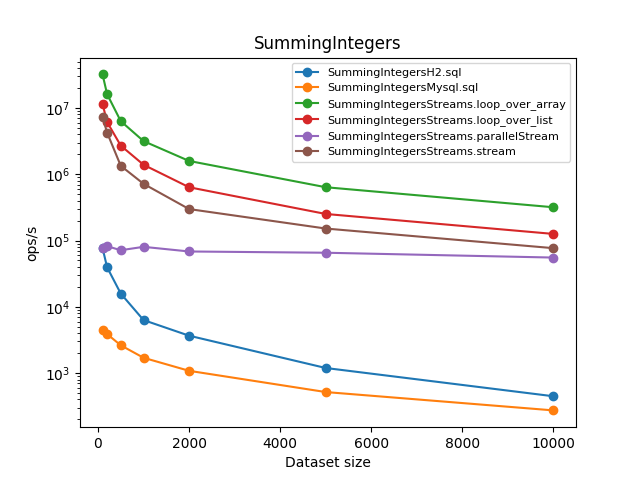
\includegraphics[width=15cm]{plots/SummingIntegers}
\caption{SummingIntegers}
\end{figure}

    Test \texttt{SummingIntegers} pokazuje wyraźnie typowe wydajności poszczególnych metod dostępu do danych. Najszybszy dostęp uzyskać można do zwykłej tablicy typu prostego, nieco wolniejsze okazują się listy (tutaj typ \texttt{ArrayList}). Dla małych zbiorów danych strumienie sekwencyjne są nawet kilka rzędów wielkości szybsze od strumieni równoległych, co nie jest zaskakujące, biorąc pod uwagę spory narzut tworzenia struktur kontrolujących przetwarzanie równoległe. Baza H2 i MySQL dla tak prostego testu mają zbyt duże narzuty, aby konkurować z pozostałymi metodami.

\newpage
\begin{figure}[H]
\centering
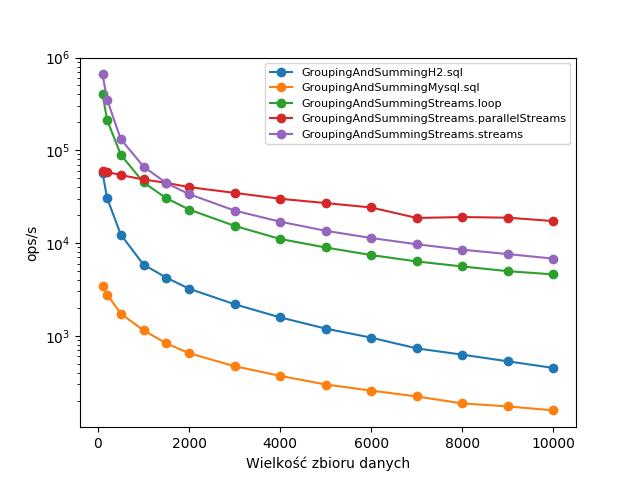
\includegraphics[width=15cm]{plots/GroupingAndSumming}
\caption{GroupingAndSumming}
\end{figure}

    Test \texttt{GroupingAndSumming} w bardzo jasny sposób ukazuje przewagę strumieni równoległych dla większych zbiorów danych i zadań, w których możliwy jest dobry podział podzadań. Strumienie typu \texttt{.parallel} okazują się szybsze od zwykłych pętli, co z jednej strony może dziwić, biorąc pod uwagę wyniki innych testów, ale z drugiej strony pokazuje, dla jakiego typu problemów strumienie są dobrym rozwiązaniem.

\newpage
\begin{figure}[H]
\centering
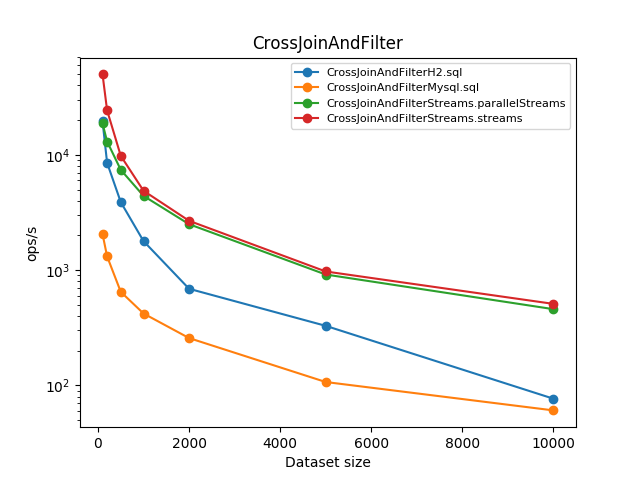
\includegraphics[width=15cm]{plots/CrossJoinAndFilter}
\caption{CrossJoinAndFilter}
\end{figure}

    Przykład \texttt{CrossJoinAndFilter} dobrze pokazuje, dla jakich typów danych przetwarzanie równoległe nie jest przydatne. Tradycyjne złączenia strumieni nie są zbyt wydajne (propozycja lepszego rozwiązania znajduje się w rozdziale X), tak więc wsparcie się równoległością prowadzi jedynie do niewielkiego zysku wydajnościowego.


\newpage
\begin{figure}[H]
\centering
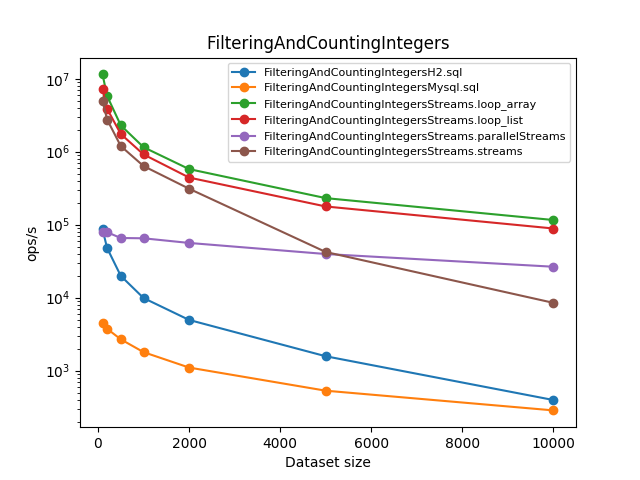
\includegraphics[width=15cm]{plots/FilteringAndCountingIntegers}
\caption{FilteringAndCountingIntegers}
\end{figure}

    Wyniki testu są bardzo podobne do testu \texttt{GroupingAndSumming}, bardzo dobrze widoczna jest przewaga strumieni równoległych nad sekwencyjnymi przy przekroczeniu pewnego rozmiaru danych wejściowych.

\newpage
\begin{figure}[H]
\centering
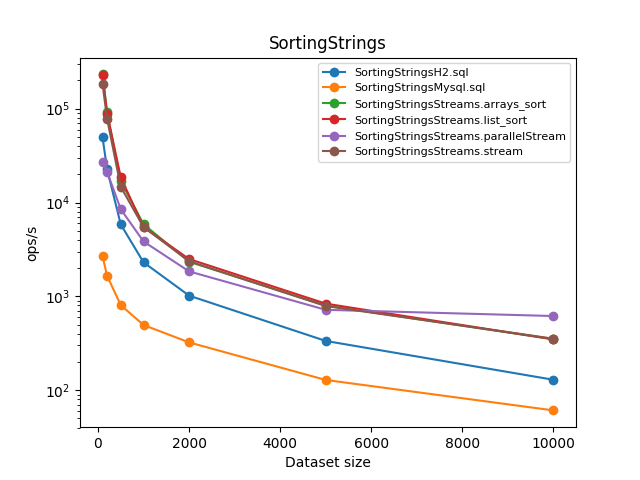
\includegraphics[width=15cm]{plots/SortingStrings}
\caption{SortingStrings}
\end{figure}

    Bardzo ciekawe zachowanie można zaobserwować w teście \texttt{SortingStrings} - dla małego rozmiaru danych wejściowych, wydajność sortowania jest bardzo zbliżona. Jest to prawdopodobnie związane z wykorzystaniem tego samego algorytmu sortowania w przypadkach, dla których wykresy praktycznie nachodzą na siebie (sortowanie tablicy, listy i sortowanie przy użyciu strumieni sekwencyjnych).

\newpage

\subsection{Podsumowanie wyników testów}

    Już po pobieżnym spojrzeniu na wyniki testów rzuca się w oczy kilka wniosków. Najszybszą i zarazem najprostszą ciągła strukturą danych jest zwykła tablica typu prostego. Ze względu na zachowanie ciągłości w pamięci (w typowych implementacjach) i najszybszym możliwym czasie dostępu do elementów z bardzo niskim poziomem abstrakcji, proste operacje wymagające sekwencyjnego odczytu są najszybsze spośród porównanych. Czasy sumowania liczb w tablicy, w porównaniu do czasów sumowania liczb w liście są średnio 3 razy mniejsze. Należy jednak zaznaczyć, że optymalizacje tego typu znacząco utrudniają pisanie kodu, ze względu na rezygnację z wygodnych metod interfejsu \texttt{List<T>}. W większości typowych, biznesowych zastosowań mikrooptymalizacje tego typu nie będą istotne z punku widzenia wydajności całych aplikacji, aczkolwiek w pewnych szczególnych zastosowaniach (np. dziedzina \textit{High Frequency Trading}) mogą mieć pewne znaczenie.

    W zbadanych przypadkach strumienie równoległe wykazują większą wydajność niż strumienie sekwencyjne od pewnego rozmiaru danych wejściowych. Utworzenie strumienia równoległego i jego skonsumowanie wymaga uruchomienie całego procesu podziału danych na wątki, wykonywania operacji i łączenia wyników z poszczególnych wątków. Daje to pewien narzut, który jest szczególnie widoczny przy małych listach, dla których operacje sekwencyjne wykonują się szybciej. Niestety, nie istnieje sposób pozwalający przewidzieć, który rodzaj strumienia (sekwencyjny czy równoległy) byłby lepszym wyborem dla danej sytuacji. Możliwe byłoby zaproponowanie heurystycznej metody, określającej rodzaj na podstawie wielkości danych wejściowych, ale nie byłby on niezawodny, więc dobór metody pozostawiony jest programiście.

    Strumienie i bezpośrednie operacje na pamięciowych strukturach języka Java są w zdecydowanej większości przypadków szybsze niż ich odpowiedniki w języku SQL. Porównując zaś bazy H2 i MySQL, testy na bazie H2 wykonywane były średnio 1.5-20 razy szybciej niż w przypadku MySQL.  Do połączenia się z bazą dyskową wykorzystany został, tak jak w przypadku bazy pamięciowej, standardowy interfejs JDBC, który wykorzystywał połączenie TCP. Przepustowość tego połączenia nie powinna mieć zbytniego znaczenia (prędkość połączenia typu loopback determinowana jest głównie przez moc procesora, a ilość danych przesyłanych jest znikoma), większy wpływ ma złożoność systemu bazodanowego i metody składowania danych. Należy zauważyć, że w przypadku największych zbiorów testowych różnice w wydajności nie przekraczają 2-3 razy. Jest to z związane z przystosowaniem i optymalizacjami baz dyskowych.


\cleardoublepage
\section{Testy wydajnościowe z użyciem TPC-H} \label{tpc}

    TPC-H jest testem referencyjnym stworzonym przez organizację \textit{Transaction Processing Performance Council}, stosowanym do badania wydajności i profilowania silników bazodanowych. Składa się on z dwóch części: generatora danych testowych oraz zbioru zapytań.

\subsection{Charakterystyka testu referencyjnego TPC-H}

    Generator danych testowych \texttt{dbgen} jest konsolowym programem, służącym do generowania zbiorów danych testowych TPC-H. Schemat bazy danych zaprezentowany jest na rysunku \ref{fig:tpcschema}. Jest to typowa hurtownia danych, gromadząca informacje o produktach, klientach, dostawcach i zamówieniach. Dokładny sens biznesowy wygenerowanych danych nie jest zbyt istotny w rozważaniach wydajnościowych, na potrzeby niniejszej pracy zakłada się ich poprawność w sensie spójności referencyjnej. Ważny jest też fakt, że dane te w przybliżeniu modelują możliwą do zaistnienia w rzeczywistości sytuację. Program \texttt{dbgen} pozwala na zdefiniowanie wielkości wygenerowanego zbioru, procentowo względem zbioru referencyjnego (100\%) o ściśle zdefiniowanym rozmiarze. Ze względu na praktyczne ograniczenia platformy testowej (16 GiB RAM), konieczne było ograniczenie maksymalnej wielkości zbioru do ok. 20-30\%, zależnie od przypadku testowego. 

    Drugą częścią TPC jest zbiór 22 zapytań testowych, z których każde odpowiada na pewne pytanie biznesowe, a na postawie odpowiedzi możliwe jest wspieranie decyzji biznesowych. Różnią się one znacznie stopniem skomplikowania (pod względem ogólnej złożoności kodu SQL) i średnim czasem wykonania. Prawidłowe wyniki wzorcowe są także udostępniane przez TPC, niestety jedynie dla zbioru danych o~wielkości 100\%. Część zapytań można jednak zwalidować mimo tego, jeśli bazują one na typowych agregacjach typu suma, średnia czy ilość - jako iż generowane dane wykazują się rozkładem jednostajnym, możliwe jest przeskalowanie sum i zliczeń względem współczynnika wielkości zbioru, jak i odpowiednie zinterpretowanie średnich. Nie jest to oczywiście zbyt pewny sposób, tak więc do środowiska badawczego wprowadzono zbiór testów jednostkowych, które sprawdzają, czy wyniki uzyskane z wykonania zapytania na wszystkich systemach bazodanowych są identyczne.

\begin{figure}
\centering
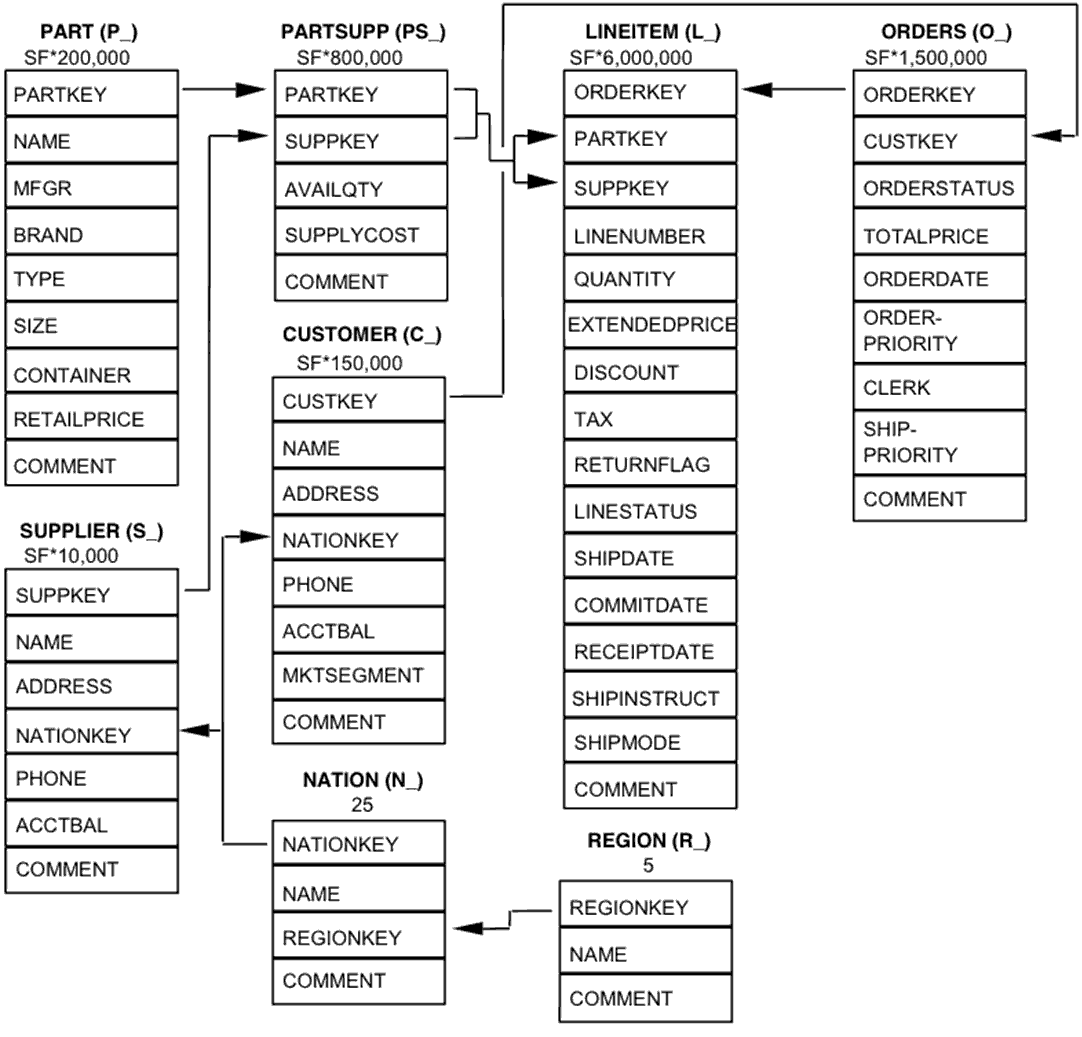
\includegraphics[width=14cm]{tpc-schema.png}
\caption{Schemat bazy danych TPC-H}
\label{fig:tpcschema}
\end{figure}


\subsection{Odwzorowanie modelu TPC}

    Aby umożliwić badanie działania strumieni na zbiorze danych testu TPC, konieczne jest przekształcenie relacyjnego modelu danych w model, który jest możliwy do zaprezentowania w języku Java. Typowe odwzorowanie stosowane w systemach obiektowo-relacyjnych wykorzystuje pola obiektów do reprezentacji kolumn oraz referencje do obiektów do reprezentacji powiązań (kluczy obcych) pomiędzy tabelami. Zastosowano więc powyższy sposób do odwzorowania oryginalnej struktury. W rezultacje wynikowy model obiektowy jest bardzo podobny do modelu relacyjnego. Jedyną różnicą jest powiązanie kolekcji \texttt{Partsupp} z kolekcją \texttt{Lineitem} - zbiory te posiadają klucz główny będący kombinacją dwóch pól. Ze względu na dość powolny proces importu danych i budowania kolekcji, konieczne stało się dodanie do klasy \texttt{Partsupp} nowego pola, będącego złączeniem powyższych dwóch pól. Poza procesem wczytywania danych, złączony klucz główny nie jest wykorzystywany.

    Cała hurtownia danych reprezentowana jest przez obiekt klasy \texttt{Store}, który przechowuje wszystkie kolekcje danych TPC. Przy implementacji importu danych okazało się, że nie ma praktycznej możliwości wykorzystania zwykłych list jako kontenerów danych. Import był bardzo powolny, ponieważ wyszukiwanie encji na podstawie kluczy w zwykłych listach wymaga przejrzenia całej listy. W związku z tym zdecydowano się w większości miejsc na wykorzystanie kolekcji mieszającej \texttt{HashMap}, w której jako klucze wykorzystano klucze główne obiektów, ze względu na ich unikalność. Z drugiej strony, nie wykorzystuje się właściwości mieszających przy badaniu wydajności strumieni, ponieważ założeniem jest, by właściwości strumieni były badane w izolacji, bez wpływu wykorzystanych struktur danych.


\subsection{Implementacja zapytań TPC przy użyciu Stream API}

Zapytania TPC w większości charakteryzują się bardzo dużą złożonością kodu oraz wykorzystaniem skomplikowanych złączeń tabel. Do implementacji wybrano kilka kwerend, kierując się stopniem skomplikowania i liczbą złączeń. Starano się zachować jak największe podobieństwo do kodu SQL, przy wykorzystaniu istniejących odpowiedników w Stream API. Niestety, w kilku przypadkach konieczne było ręczne zaimplementowanie operacji nie mających odzwierciedlenia w strumieniach, np. funkcje agregujące operujące na kilku kolumnach jednocześnie. Spowodowało to znaczne rozrośnięcie się ilości kodu i znaczący spadek jego czytelności. 

    Dodatkowo, wprowadzono zbiór testów jednostkowych, weryfikujących zgodność wyników zapytań dla wszystkich metod dostępu do danych. Referencyjne wyniki \cite{tpcresults} udostępniane przez konsorcjum TPC mają zastosowanie jedynie dla zbioru danych generowanego z współczynnikiem 1.0, więc konieczne jest wprowadzenie innej metody weryfikacji poprawności wyników. Jako iż postać wyniku zapytania w~przypadku wszystkich metod jest identyczna, nie było problemem zaimplementowanie kilku prostych testów dla każdej metody przetwarzania danych.


\newpage
\subsection{Wyniki} \label{tpcgraphs}

\begin{figure}[h]
\centering
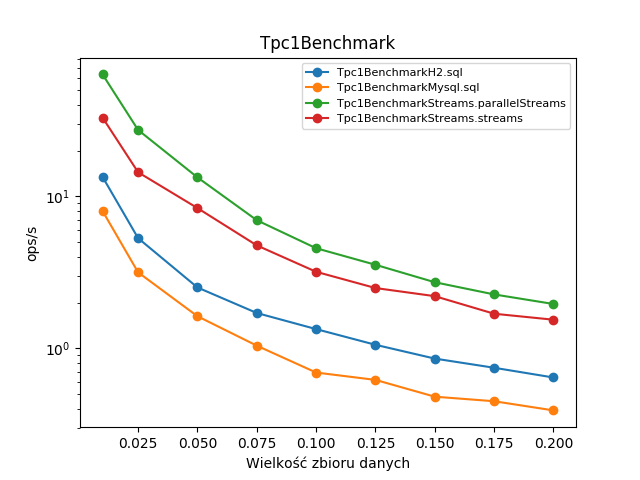
\includegraphics[width=15cm]{plots/Tpc1Benchmark}
\caption{Tpc1Benchmark}
\end{figure}

    Zapytanie nr 1 obejmowało filtrowanie i wielokrotne wykorzystanie funkcji agregujących \texttt{sum}, \texttt{avg} i \texttt{count}. Przy większych rozmiarach zbioru danych strumienie wykazują większą liczbę operacji na sekundę, a związane to jest z bardzo łatwym zrównoleglaniem operacji agregujących, w których łączenie pośrednich kontenerów danych w implementacji interfejsu \texttt{Collector} jest bardzo szybkie. W zakresie baz SQL, baza pamięciowa prezentuje w tym przypadku większą wydajność, przy czym dla każdej wielkości zbioru testowego baza pamięciowa jest lepsza od bazy dyskowej. 

\newpage
\begin{figure}[H]
\centering
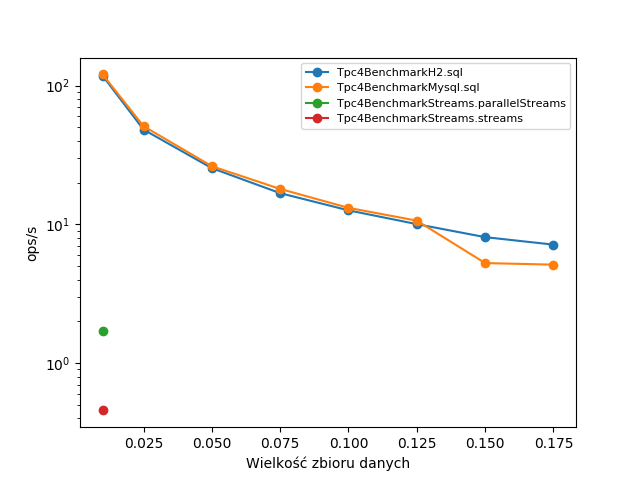
\includegraphics[width=15cm]{plots/Tpc4Benchmark}
\caption{Tpc4Benchmark}
\end{figure}

    Wyniki testów dla zapytania nr 4 prezentują bardzo wyraźnie możliwości silnika SQL w zakresie optymalnej interpretacji zapytania zagnieżdżonego (\textit{inner query}) i jego efektywnego wykonania. W przypadku implementacji strumieniowej, zapytanie zagnieżdżone jest zapisane w postaci funkcji wewnętrznej, która wykazuje te same problemy wydajnościowe, co złączenia kolekcji. W przypadku strumieni nie przeprowadzono badań wydajnościowych dla wielu wielkości zbioru danych, ze względu na skrajnie wolne wykonywanie się testu.

\newpage
\begin{figure}[H]
\centering
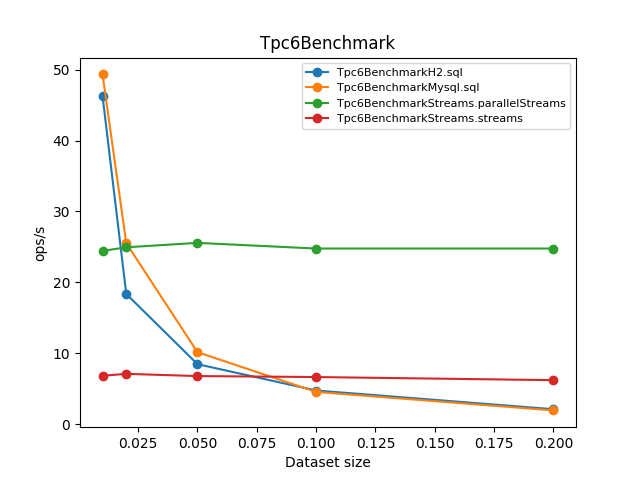
\includegraphics[width=15cm]{plots/Tpc6Benchmark}
\caption{Tpc6Benchmark}
\end{figure}

    Zapytanie nr 6 jest bardzo podobne do zapytania nr 1, ponieważ także obejmuje jedną tabelę, ale tylko jedną funkcję agregującą. Podobnie jak w teście nr 1, w tak prostym przypadku strumienie wykazują większą wydajność, przy czym strumienie równoległe prezentują się znacznie lepiej niż strumienie sekwencyjne. Taka przewaga jest zawsze widoczna przy operacjach łatwych do podzielenia i zrównoleglenia wzorcem FJP.

\newpage
\begin{figure}[H]
\centering
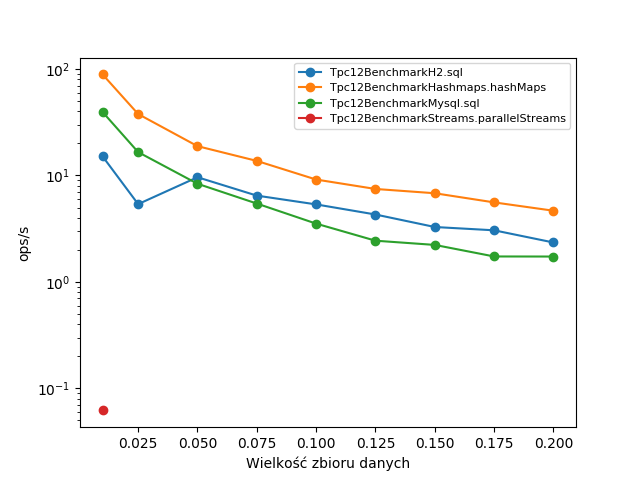
\includegraphics[width=15cm]{plots/Tpc12Benchmark}
\caption{Tpc12Benchmark}
\end{figure}

    Test nr 12 pokazuje, jak nieefektywna jest najprostsza metoda łączenia strumieni, przy wykorzystaniu metody \texttt{Stream.flatMap}. Duża aktywność odśmiecacza pamięci spowodowana ciągłym tworzeniem obiektów reprezentujących iloczyn kartezjański wpływa dodatkowo negatywnie na wynik. Bazy relacyjne reprezentują znacznie większą prędkość wykonywania zapytania, natomiast najlepszym rozwiązaniem okazuje się ręcznie zaimplementowany operator złączenia naturalnego, bazujący na kolekcjach mieszających. Podobnie jak w przypadku testu nr 4, nie przeprowadzony wszystkich testów ze względu na długi czas wykonania.

\newpage
\begin{figure}[H]
\centering
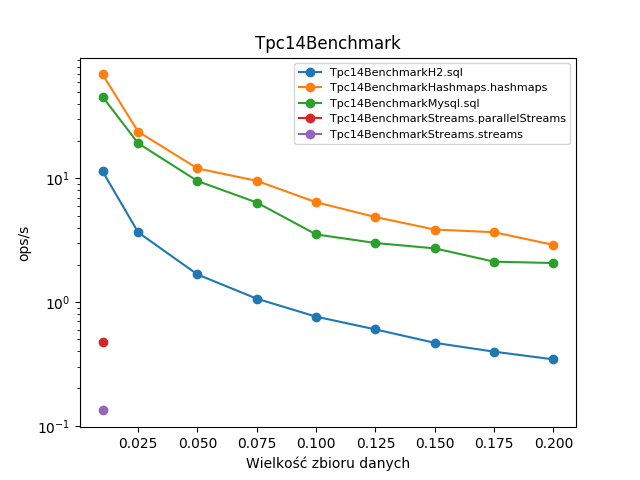
\includegraphics[width=15cm]{plots/Tpc14Benchmark}
\caption{Tpc14Benchmark}
\end{figure}

    Ostatni test nr 14 potwierdza znakomitą wydajność bazy MySQL w zakresie operacji łączenia tabel, przy czym baza H2 jest jedynie kilka razy wolniejsza. Funkcje agregujące mogą być bardzo efektywnie wykonywane w przypadku jednoczesnego złączenia tabel.

\newpage
\begin{figure}[H]
    \centering
    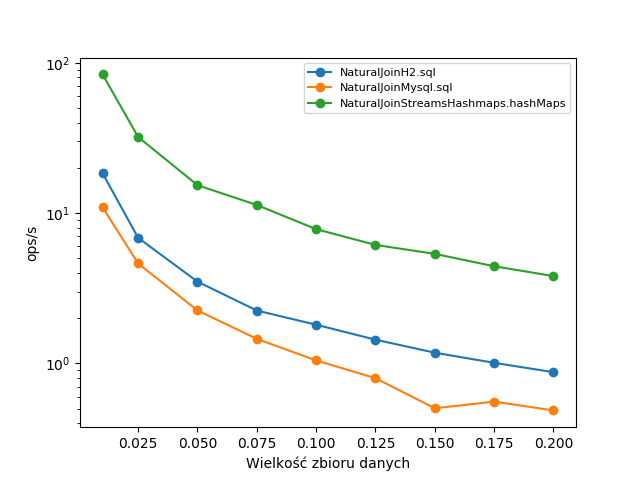
\includegraphics[width=13cm]{plots/NaturalJoin}
    \caption{Porównanie wydajności złączenia naturalnego}
    \label{fig:naturaljoingraph}
\end{figure}

Niniejszy wykres obrazuje porównanie szybkości wykonywania się złączenia kolekcji \texttt{LineItem} i \texttt{Order} na podstawie odpowiedniego klucza głównego. Jak można zaobserwować, kolekcja haszująca zapewnia bardzo szybkie wyszukiwanie obiektów przy podaniu klucza, więc przy założeniu jego unikalności połączenie dwóch zbiorów w pamięci jest znacznie szybsze niż wykonanie tego samego zadania czy to w bazie dyskowej, czy w bazie pamięciowej H2. Narzut struktur danych bazy pamięciowej jest tutaj wyraźnie widoczny.

\subsection{Podsumowanie wyników testów TPC}

    Wyniki testów referencyjnych nie wskazują jednoznacznie na najlepsze rozwiązanie do użycia w każdym przypadku. Praktycznie każdy test prezentuje cechy wydajnościowe metod dostępu do danych w innym kontekście. Wiele tłumaczy ściśle relacyjny charakter zbioru testowego TPC. Duża liczba tabel i powiązań między nimi powoduje, że zapytania strumieniowe zawierające złączenia są zwykle znacznie mniej wydajne od prostszych zapytań operujących na jednej tabeli. Prawdopodobnie wykorzystanie innego zbioru danych, charakteryzującego się mniejszą normalizacją i większą nadmiarowością przyniosłoby inne wyniki. 

    Zapytania zagnieżdżone są sporym problemem dla przetwarzania strumieniowego. W bazach SQL planista zapytania jest w stanie dokonać analizy kodu i dokonać odpowiednich optymalizacji. W przypadku strumieni żadne tego typu optymalizacje nie występują i nie są możliwe do implementacji w prosty sposób, ponieważ wszystkie funkcje strumieniowe wykonują się w izolacji przez wewnętrzne struktury biblioteki. O ile użycie równoległej odmiany strumieni jest w stanie zwiększyć nieco szybkość przetwarzania, nie są to znaczne przyrosty.


\subsection{Porównanie ilości zajętej pamięci}

    W ramach badania wydajności metod dostępu do danych postanowiono dodatkowo sprawdzić ilość pamięci, wykorzystywanej przez bazy danych do ich przechowywania. Jak przewidywano, baza dyskowa MySQL przechowuje dane na dysku w najbardziej kompaktowej postaci. Schemat TPC w postaci obiektów znajdujących się w pamięci maszyny wirtualnej zajmuje więcej miejsca, natomiast w przypadku bazy pamięciowej H2 zaobserwować można pewien narzut wewnętrznych struktur danych.

\begin{figure}[H]
\centering
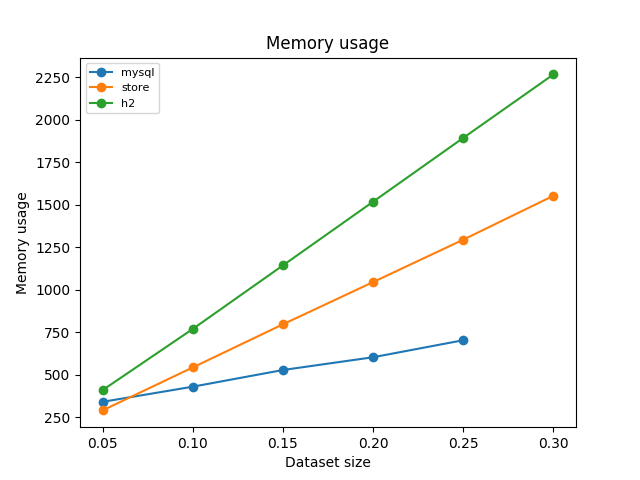
\includegraphics[width=13cm]{plots/memory}
\caption{Tpc14Benchmark}
    \label{fig:memoryconsumption}
\end{figure}
    

\cleardoublepage
\section{Podsumowanie}


Celem pracy było przeprowadzenie analizy porównawczej możliwości przetwarzania danych w pamięciowych bazach SQL i przy użyciu Stream API w Java 8. Cel został osiągnięty. Przeprowadzono szczegółowe badania wydajnościowe przy użyciu zarówno losowych danych testowych, jak i przy użyciu testu referencyjnego TPC, korzystając z odpowiednio skonstruowanego środowiska badawczego i przy wykorzystaniu odpowiednich narzędzi programowych. Środowisko badawcze pozwala na powtórzenie badań na dowolnie wybranej platformie sprzętowej spełniającej wymagania. Dokonano porównania dwóch metod dostępu do danych w zakresie języka programowania, sposobu konstruowania zapytań jak i możliwości języka zapytań.

    Stream API w połączeniu z wyrażeniami lambda jest bardzo przydatną nowością wprowadzoną w Javie 8. Wprowadzone niewielkie części paradygmatu funkcyjnego pozwalają na pisanie wydajnego i łatwo testowalnego kodu. Strumienie są bardzo dobrą alternatywą dla tradycyjnych elementów składni języka, takich jak pętle i~warunki, które można zastąpić metodami Stream API. Z drugiej strony, strumienie sprawdzają się najlepiej na pojedynczych kolekcjach jednorodnych obiektów, łączenie wielu kolekcji charakteryzujących się typowo relacyjną strukturą nie jest wspierane domyślnie i okazuje się, jak wykazały badania, znacznie utrudnione. Tworzenie skomplikowanych sekwencji operacji, zwłaszcza własnoręcznie definiowanych, jest zdecydowanie bardziej skomplikowane i wymaga znacznie więcej kodu niż w języku SQL, który do takich operacji został stworzony. Możliwe jest osiągnięcie znacznych szybkości wykonywania zapytań SQL w pamięci, natomiast należy mieć na uwadze, że wydajność nie jest najważniejszą rzeczą w systemie bazodanowym. Należy zwrócić uwagę na wsparcie producentów, narzędzia wspomagające (np. analizatory planu zapytań) i bezpieczeństwo (kopie zapasowe, metody replikacji), ponieważ w~ogólnym rozrachunku elementy te mogą mieć większe znaczenie.

    Strumienie doskonale nadają się do prostego, równoległego przetwarzania danych, pod warunkiem, że całe zadanie daje się łatwo rekurencyjnie podzielić na mniejsze podzadania, a szybkość wykonywania zależna jest od mocy obliczeniowej procesora. W typowych przypadkach sama zmiana strumienia z domyślnego sekwencyjnego na równoległy może przynieść kilkukrotny wzrost wydajności. Należy jednak zwrócić uwagę, iż strumienie równoległe mają pewien narzut, który, w przypadku małych zbiorów danych, bądź zbyt małej ilości pracy do wykonania w podzadaniu, może okazać się większy, niż narzut strumieni sekwencyjnych. Warto więc zawsze badać, czy próba optymalizacji na pewno przyniesie oczekiwane efekty.



    Jednym z największych wyzwań było zaproponowanie i zaimplementowanie rozwiązania, pozwalającego na import danych bazy testowej TPC zarówno do środowiska bazy SQL, jak i do modelu danych w pamięci wykorzystywanego przez Stream API. Różnice w sposobie dodawania danych, jak i w sposobie ich odczytu wymagały przemyślenia struktury rozwiązania, a następnie napisania dużej ilości pomocniczego kodu pośredniczącego. Pojawiły się poważne problemy wydajnościowe, związane z~ prędkością importowania danych do bazy MySQL przez dużą liczbę kwerend \texttt{SELECT}. Konieczne okazało się opakowanie narzędzia importującego \texttt{mysqlimport} i zintegrowanie go z istniejącym kodem Java.

    Technicznym problemem, który pojawił się na samym początku budowy środowiska testowego, było umożliwienie wykonywania metod przeznaczonych do badania zarówno poprzez narzędzie JMH, jak i w testach jednostkowych JUnit. Specificzna budowa klasy testu referencyjnego (m. in. automatyczna, zewnętrzna parametryzacja), wspierająca łatwe wykonywanie prostych badań, okazała się bardzo problematyczna w zakresie możliwości jej użycia poza kontekstem JMH. Konieczne było znalezienie sposobu, w którym kolejne wywołania metod z klasy testu referencyjnego nie naruszają logicznej struktury kodu i umożliwiają wyciągnięcie, a następnie porównanie wyników wszystkich typów testów.

    Generowanie danych pseudolosowych było konieczne do implementacji testów operujących na danych syntetycznych. Okazało się, że testowanie poprawności wyników zapytań dla wszystkich metod dostępu do danych jest niemożliwe, jeśli generator dostarcza różne dane przy kolejnych jego uruchomieniach. Ze względu na chęć uzyskania jak największej powtarzalności, wykorzystano stałe ziarno generatora losowego \texttt{java.util.Random}.


    W dalszych pracach nad porównaniem możliwości przetwarzania pamięciowego jednym z pomysłów jest zbadanie baz NoSQL działających w pamięci. Rozwiązania nierelacyjne posiadają wiele cech niespotykanych w tradycyjnych bazach SQL, takich jak brak ściśle zdefiniowanego schematu czy praca w modelu rozproszonym (\textit{sharding}). Być może cechy te przekładają się na wydajność czy sposób formułowania kodu aplikacji w taki sposób, że rozwiązanie typu NoSQL będzie miało przewagę nad analizowanymi w niniejszej pracy rozwiązaniami.

    Stream API jest bardzo wygodnym interfejsem programistycznym, którego zakres widoczny przez końcowego użytkownika jest niewielki. Szczegóły implementacyjne, takie jak interfejs \texttt{Spliterator} pozwalający na dokładne zdefiniowanie sposobu podziału zadań na wątki, czy realizacja przydziału zadań do wątków, mogą być istotnym tematem do analizy. Możliwe, że odpowiednie zrozumienie i wykorzystanie niskopoziomowych klas strumieni pozwoliłoby na dokonanie lepszych optymalizacji i w konsekwencji uzyskanie lepszych wyników. Dobrym pomysłem byłoby zaproponowanie odmiany Stream API zorientowanej na wydajność, do zastosowań podobnych jak te, o których opisuje niniejsza praca.

\cleardoublepage
\begin{thebibliography}{9}

    \bibitem{ullman} 
        J.D. Ullman, J. Widom,
        \textit{A first course in database systems}, 
        Prentice Hall, 2008

    \bibitem{linq}
        Andreq Troelsen,
        \textit{Pro C\# 5.0 and the .NET 4.5 Framework}, wyd. Apress, 2012

    \bibitem{tpcresults} 
        TPC Council,
        \textit{TPC Benchmark H Standard Specification, page 136},
        1993-2014 TPC Council

    \bibitem{orm} 
        Christian Bauer,
        \textit{Java Persistence with Hibernate},
        wyd. Manning Publications, 2015

    \bibitem{streamsjavadoc} 
        Oracle Corporation
        \textit{java.util.stream Javadoc documentation},
        http://docs.oracle.com/javase/8/docs/api/java/util/stream/package-summary.html, czas dostępu 29.05.2017

    \bibitem{latexcompanion} 
        Raoul-Gabriel Urma
        \textit{Processing Data with Java SE 8 Streams, Part 1}, 
        http://www.oracle.com/technetwork/articles/java/ma14-java-se-8-streams-2177646.html, czas dostępu 26.05.2017

    \bibitem{fjpdocs} 
        Oracle Corporation
        \textit{ForkJoinPool documentation}, 
        https://docs.oracle.com/javase/8/docs/api/java/util/concurrent/ForkJoinPool.html, czas dostępu 29.05.2017

    \bibitem{generics} 
        Oracle Corporation
        \textit{The Java Tutorials: Generics}, 
        https://docs.oracle.com/javase/tutorial/java/generics/types.html, czas dostępu 29.05.2017

    \bibitem{jdbc} 
        Oracle Corporation
        \textit{JDBC Database Access}, 
        https://docs.oracle.com/javase/tutorial/jdbc/, czas dostępu 15.06.2017

    \bibitem{goetz}
        \textit{Wypowiedź architekta języka Java, Brian Goetz}
        https://stackoverflow.com/questions/17960656/is-it-possible-to-use-java-8-streams-api-for-asynchronous-processing/18826615\#comment36545451\_18826615, czas dostępu 29.05.2017

    \bibitem{joolambda} 
        \textit{Biblioteka JOO$\lambda$}, https://www.jooq.org/products/, czas dostępu 28.05.2017

    \bibitem{streamex} 
        \textit{Biblioteka StreamEx} https://github.com/amaembo/streamex, czas dostępu 28.05.2017

    \bibitem{h2maven} 
        \textit{Informacje o pakietach bazy H2 na portalu Maven Central} https://mvnrepository.com/artifact/com.h2database/h2, czas dostępu 28.05.2017

    \bibitem{matplotlib} 
        \textit{Dokumentacja biblioteki matplotlib} https://matplotlib.org/users/pyplot\_tutorial.html, czas dostępu 15.05.2017

\end{thebibliography}

\cleardoublepage
\appendix
\section{Dokumentacja środowiska badawczego}

    Środowisko badawcze, przygotowane na potrzeby niniejszej pracy, składa się z kilku części: zawiera testy referencyjne operujące na danych syntetycznych, pełny kod narzędzia \texttt{dbgen}, testy referencyjne operujące na zbiorze danych TPC oraz skrypty do generowania wykresów i automatyzacji procesu testowania. Do poprawnego wykonywania testów powinny być spełnione następujące wymagania:
    
\begin{itemize}
    \item pamięć RAM w ilości zależnej od objętości wczytywanych danych testowych (ilość pamięci zajmowana przez zbiór TPC zaprezentowana jest na rys. \ref{fig:memoryconsumption})
    \item maszyna wirtualna Java i środowisko deweloperskie JRE w wersji 8
    \item kompilator języka C
    \item do wykonywania testów na bazie MySQL - system bazodanowy MySQL, działający na domyślnym porcie z użytkownikiem \texttt{root} i hasłem \texttt{password}
    \item do generowania wykresów - interpreter języka Python 3 i zainstalowana biblioteka matplotlib
\end{itemize}

    Ze względu na wykorzystanie skryptów Bash do automatycznego uruchamiania testów i generowania wykresów, systemy Linux i OSX są najlepiej przystosowane do wykonywania badań. Na innych systemach wspierających technologię Java wykonywanie badań jest także możliwe, przy ręcznym wykorzystaniu linii poleceń.

    Kod narzędzia \texttt{dbgen} został włączony w całości do projektu środowiska badawczego. Zbiór TPC o określonej wielkości jest tworzony na nowo przy każdym uruchomieniu testu TPC. Należy upewnić się, że jest dostępna odpowiednia ilość wolnego miejsca na dysku. Import danych testowych w celu badania wydajności strumieni wykonywany jest przy pomocy klasy \texttt{Store} i odpowiadającym tabelom klas odwzorowujących. Ładowanie danych do bazy H2 odbywa się bezpośrednio poprzez funkcję \texttt{RUNSCRIPT} i skrypt tworzący odpowiednie tabele, natomiast baza MySQL zapełniana jest zewnętrznym narzędziem \texttt{mysqlimport}.

    W pliku konfiguracyjnym \texttt{build.gradle} możliwe jest zdefiniowanie kilku parametrów narzędzia JMH, między innymi liczba grup iteracji testu, opcje tworzenia nowej instancji maszyny wirtualnej Java przy każdym teście oraz ilość przydzielonej jej pamięci. Należy mieć na uwadze, że przydzielenie zbyt małej ilości pamięci z dużym prawdopodobieństwem da nierzetelne wyniki, ze względu na wzmożoną aktywność odśmiecacza pamięci, możliwe jest też przepełnienie się pamięci i przerwanie działania. 

    Klasy testowe znajdują się w folderze \texttt{src/jmh/java/masterthesis}. Przykładowo, aby uruchomić test referencyjny \texttt{SummingIntegers} badający strumienie należy wywołać następujące polecenie:

\begin{verbatim}
$ ./gradlew clean jmh -Pinclude='SummingIntegersStreams'
\end{verbatim}

    Aby uruchomić testy sumowania liczb dla wszystkich metod dostępu do danych, należy użyć wyrażenia regularnego, które odpowiada wszystkim klasom dla danej metody:

\begin{verbatim}
$ ./gradlew clean jmh -Pinclude='SummingIntegers.*'
\end{verbatim}

    Po przeprowadzeniu testu, raport wynikowy zostanie wyświetlony na ekranie, a także zapisany do pliku \texttt{results.txt} w folderze \texttt{build}.

    Wszystkie wielkości zbiorów testowych zaszyte są w odpowiednich klasach testowych, w adnotacjach \texttt{@Param}. Możliwe jest wybranie dowolnej wielkości. Dodatkowo, dostarczony został skrypt \texttt{runall.sh} wykonujący wszystkie istniejące testy i automatycznie generujący wykresy na podstawie raportów. W celu wygenerowania pojedynczego wykresu na podstawie pliku raportu, należy wywołać polecenie:

\begin{verbatim}
$ ./plotgen.py ../build/reports/jmh/results.txt log "NazwaWykresu"
\end{verbatim}


\end{document}
